\section{Informationsverarbeitung in Natur und Technik}

\subsection{Neuroprothetik: Auslesen aus dem Gehirn}

Dies ist eigentlich kein direkter Teilbereich der Bionik, da selten Lösungen aus der Biologie in die Technik übertragen werden und stattdessen die biologischen Funktionen des Menschen durch Technische ersetzt werden. Z.B.\ Cochlea-Implantate, Retina-Implantate, Cortex-Implantate.

Beim \textit{Cochlea-Implantat} wird ein Elektrodenträger in die Hörschnecke eingebracht. Je nach Frequenz eines am Mikrofon eingehenden Tons wird eine bestimmte Elektrode aktiviert, und das Signal an die entsprechende Stelle des Innenohrs weitergegeben. Dadurch kann der Hörsinn wiederhergestellt werden.

Beim \textit{Retina-Implantant} wird ein Mikroelektroden-Raster entweder auf oder unter die Retina gesetzt und Signale werden an die optischen Nerven weitergegeben.

Bei \textit{Cortex-Implantaten} geht es darum, Signale direkt im Gehirn einzubringen. Solche Systeme ermöglichen es z.B.\ Kamerabilder direkt ins Gehirn zu schicken.

\begin{center}
    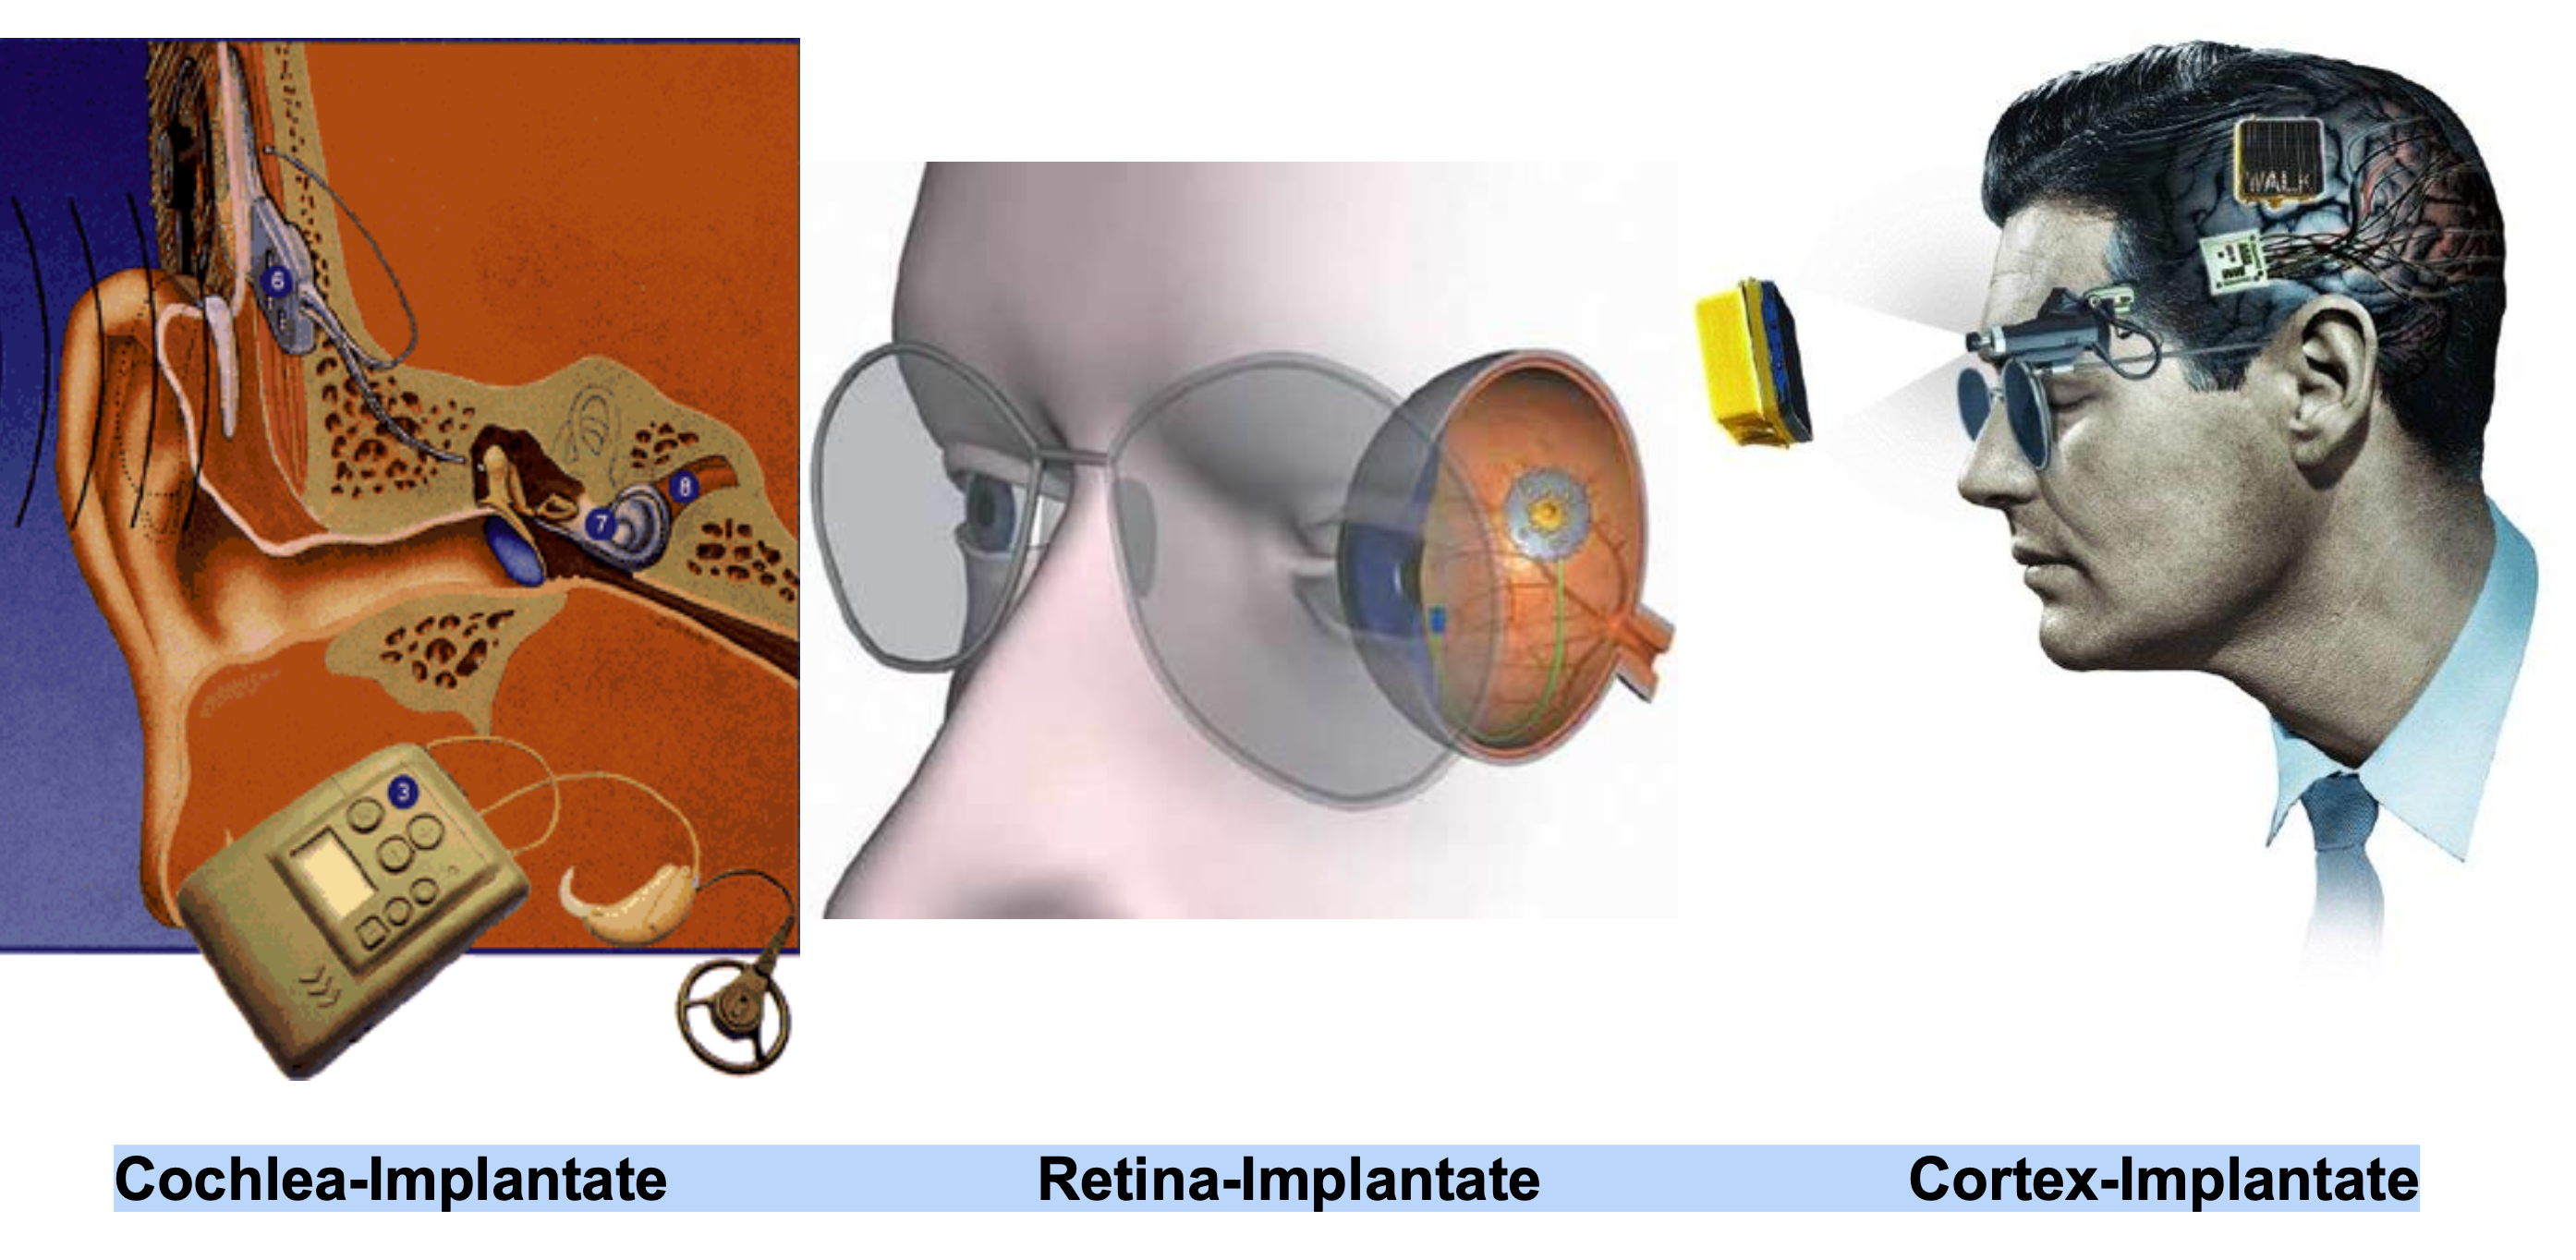
\includegraphics[width=10cm]{lec8/figures/neuroprothetik.png}
\end{center}

\subsection{Biohybridtechnik}

Hierbei geht es um die Kombination von biologischen und technischen Systemen. Ein Beispiel wäre z.B.\ die Nutzung einer biologischen Nase, um die an den Rezeptoren erzeugten Signale direkt elektronisch weiterzuverarbeiten. Allerdings ist dieser Bereich auch nicht wirklich bionisch.

\begin{center}
    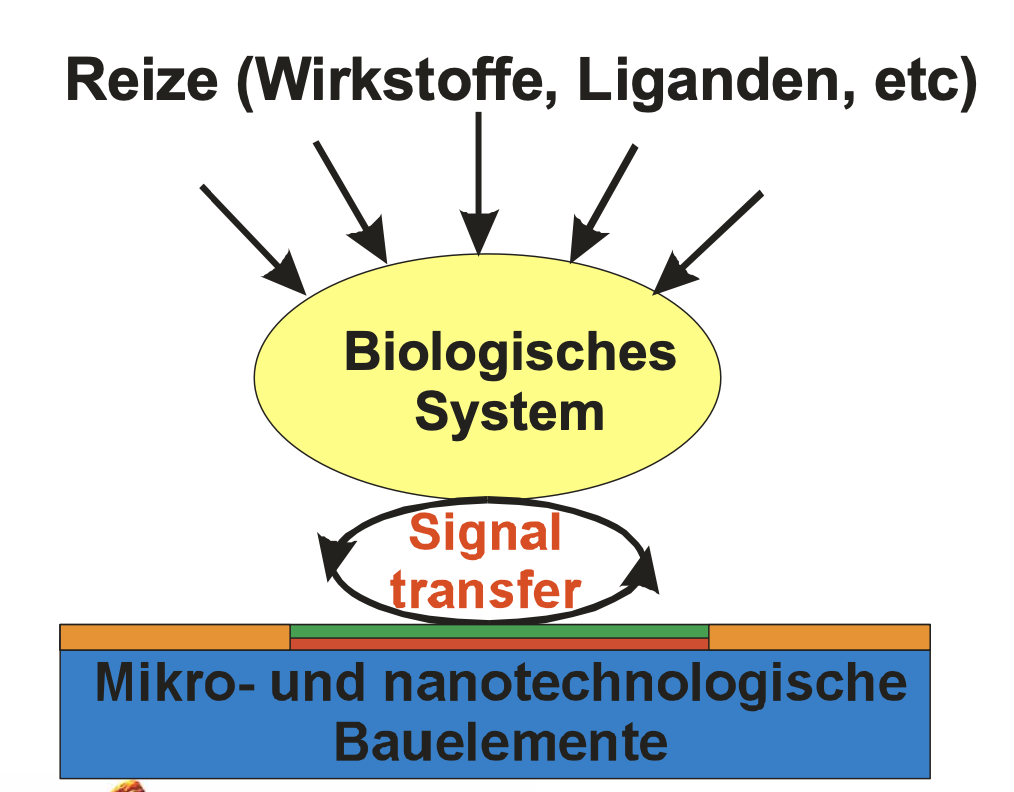
\includegraphics[width=7cm]{lec8/figures/biohybrid.png}
\end{center}

\subsection{Datenverarbeitung im Gehirn (Neurobionik i.e.S.)}

\textbf{Was können Gehirne besser als technische Informationsverarbeitungssysteme \dangersign?} Biologische Systeme kommen mit Beschränkungen aus, bspl.\ einem beeinträchtigten Seh-/Gehörsinn bei wechselhaften Umweltbedingungen. Wir möchten dies gerne auf autonome Roboter übertragen.

Organismen müssen z.B.\ auf Gefahren in Echtzeit reagieren können, weshalb die Verarbeitungsgeschwindigkeit zu Lasten der Verarbeitungsqualität optimiert ist. Dies ist möglich, da das Gehirn eingehende Signale unter der Annahme zahlreicher Regeln verarbeitet, siehe die optischen Illusionen. Bei dem Krebs wird je nach Sehwinkel der Auflösung der Augen eingeschränkt ($\rightarrow$ Datenreduktion). Zudem erkennen Hilfsmechanismen wichtige Ereignisse in der Peripherie (z.B. Bewegungen) und lösen Augenbewegungen aus, um den Fokus dorthin zu setzen (siehe im Bild rechts unten).

\begin{figure}[!h]
  \centering
  \includegraphics[width=7cm]{lec8/figures/täuschung.png}
  \hfill
  \begin{minipage}{.45\linewidth}
    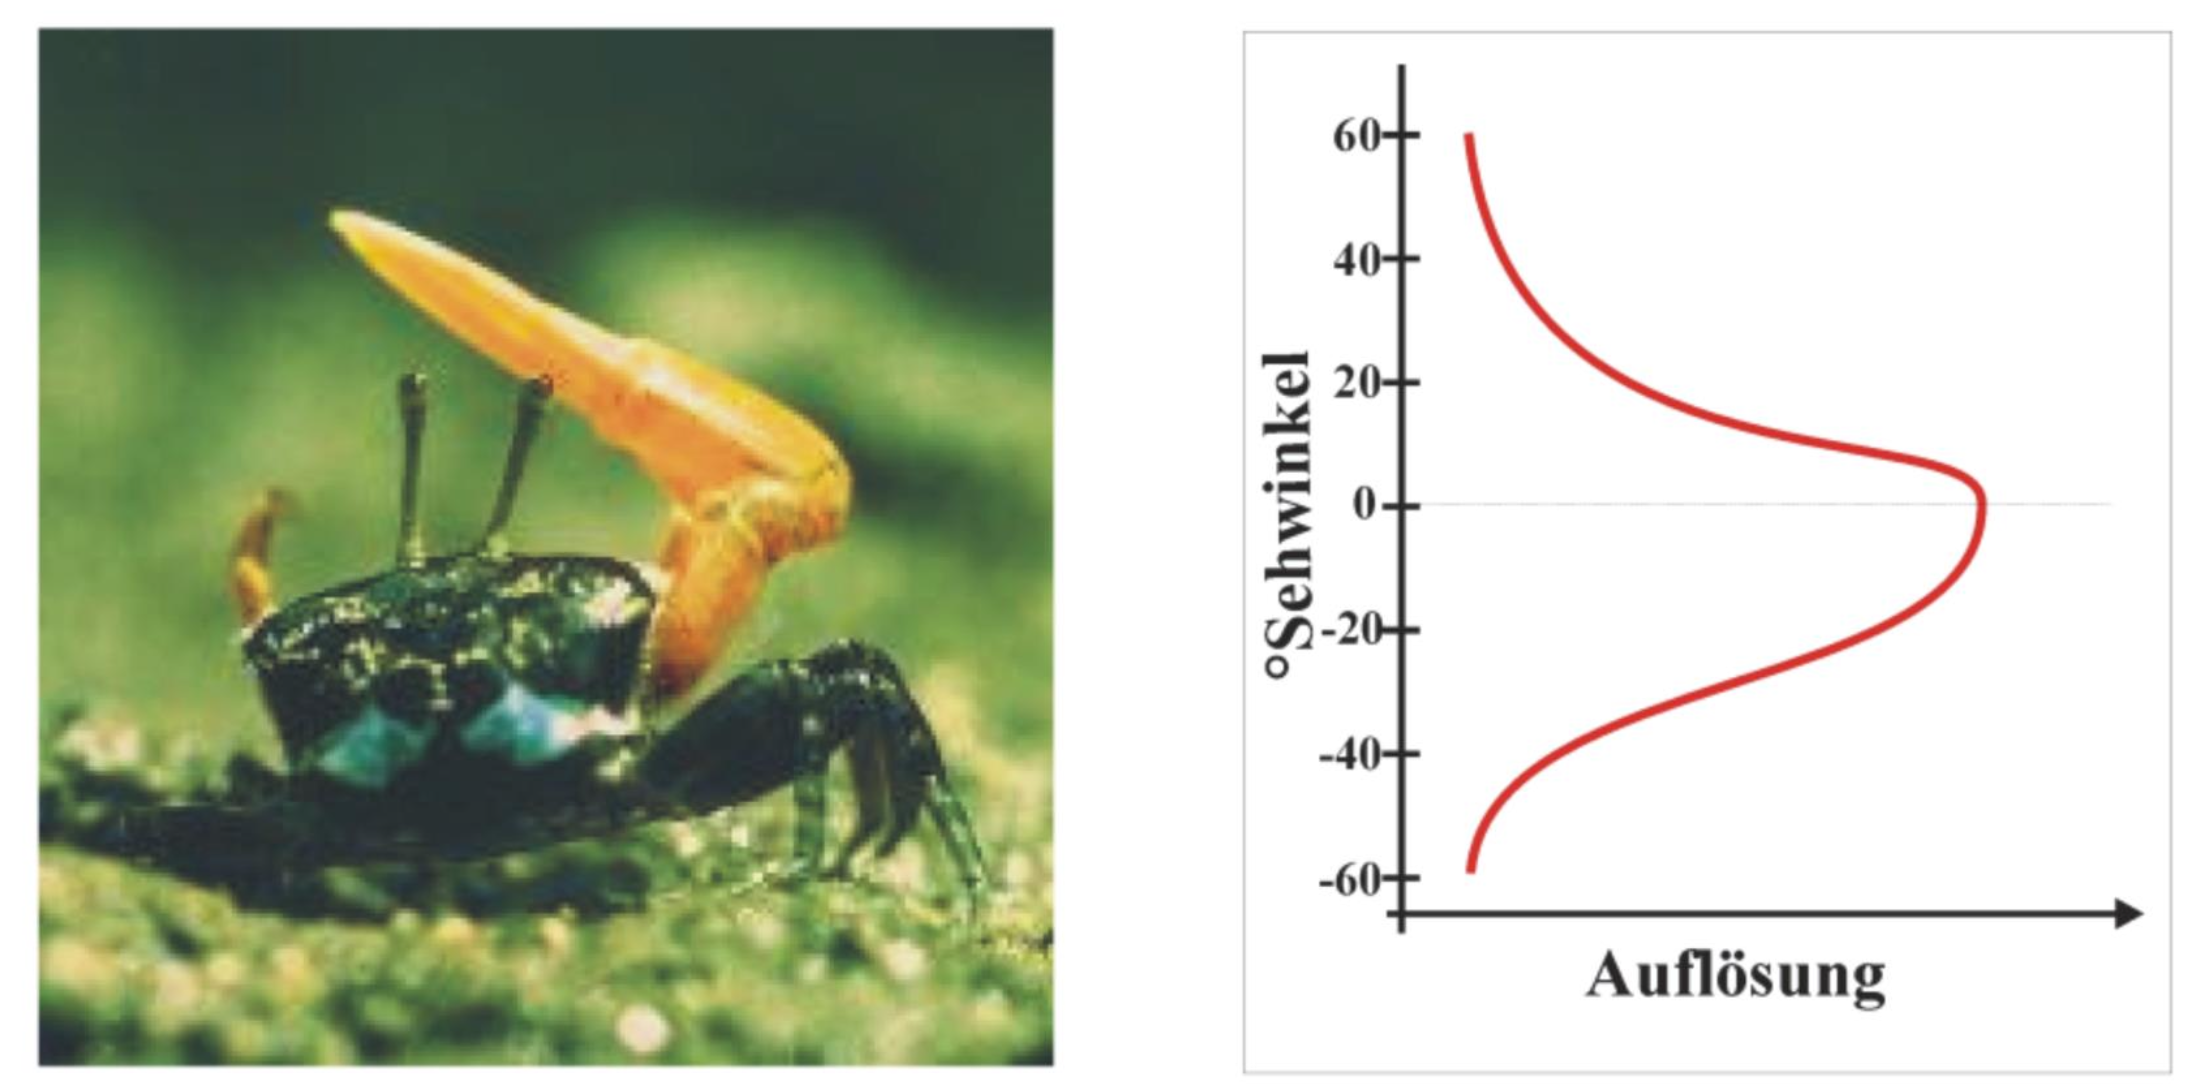
\includegraphics[width=\linewidth]{lec8/figures/krebs.png}
    \\
    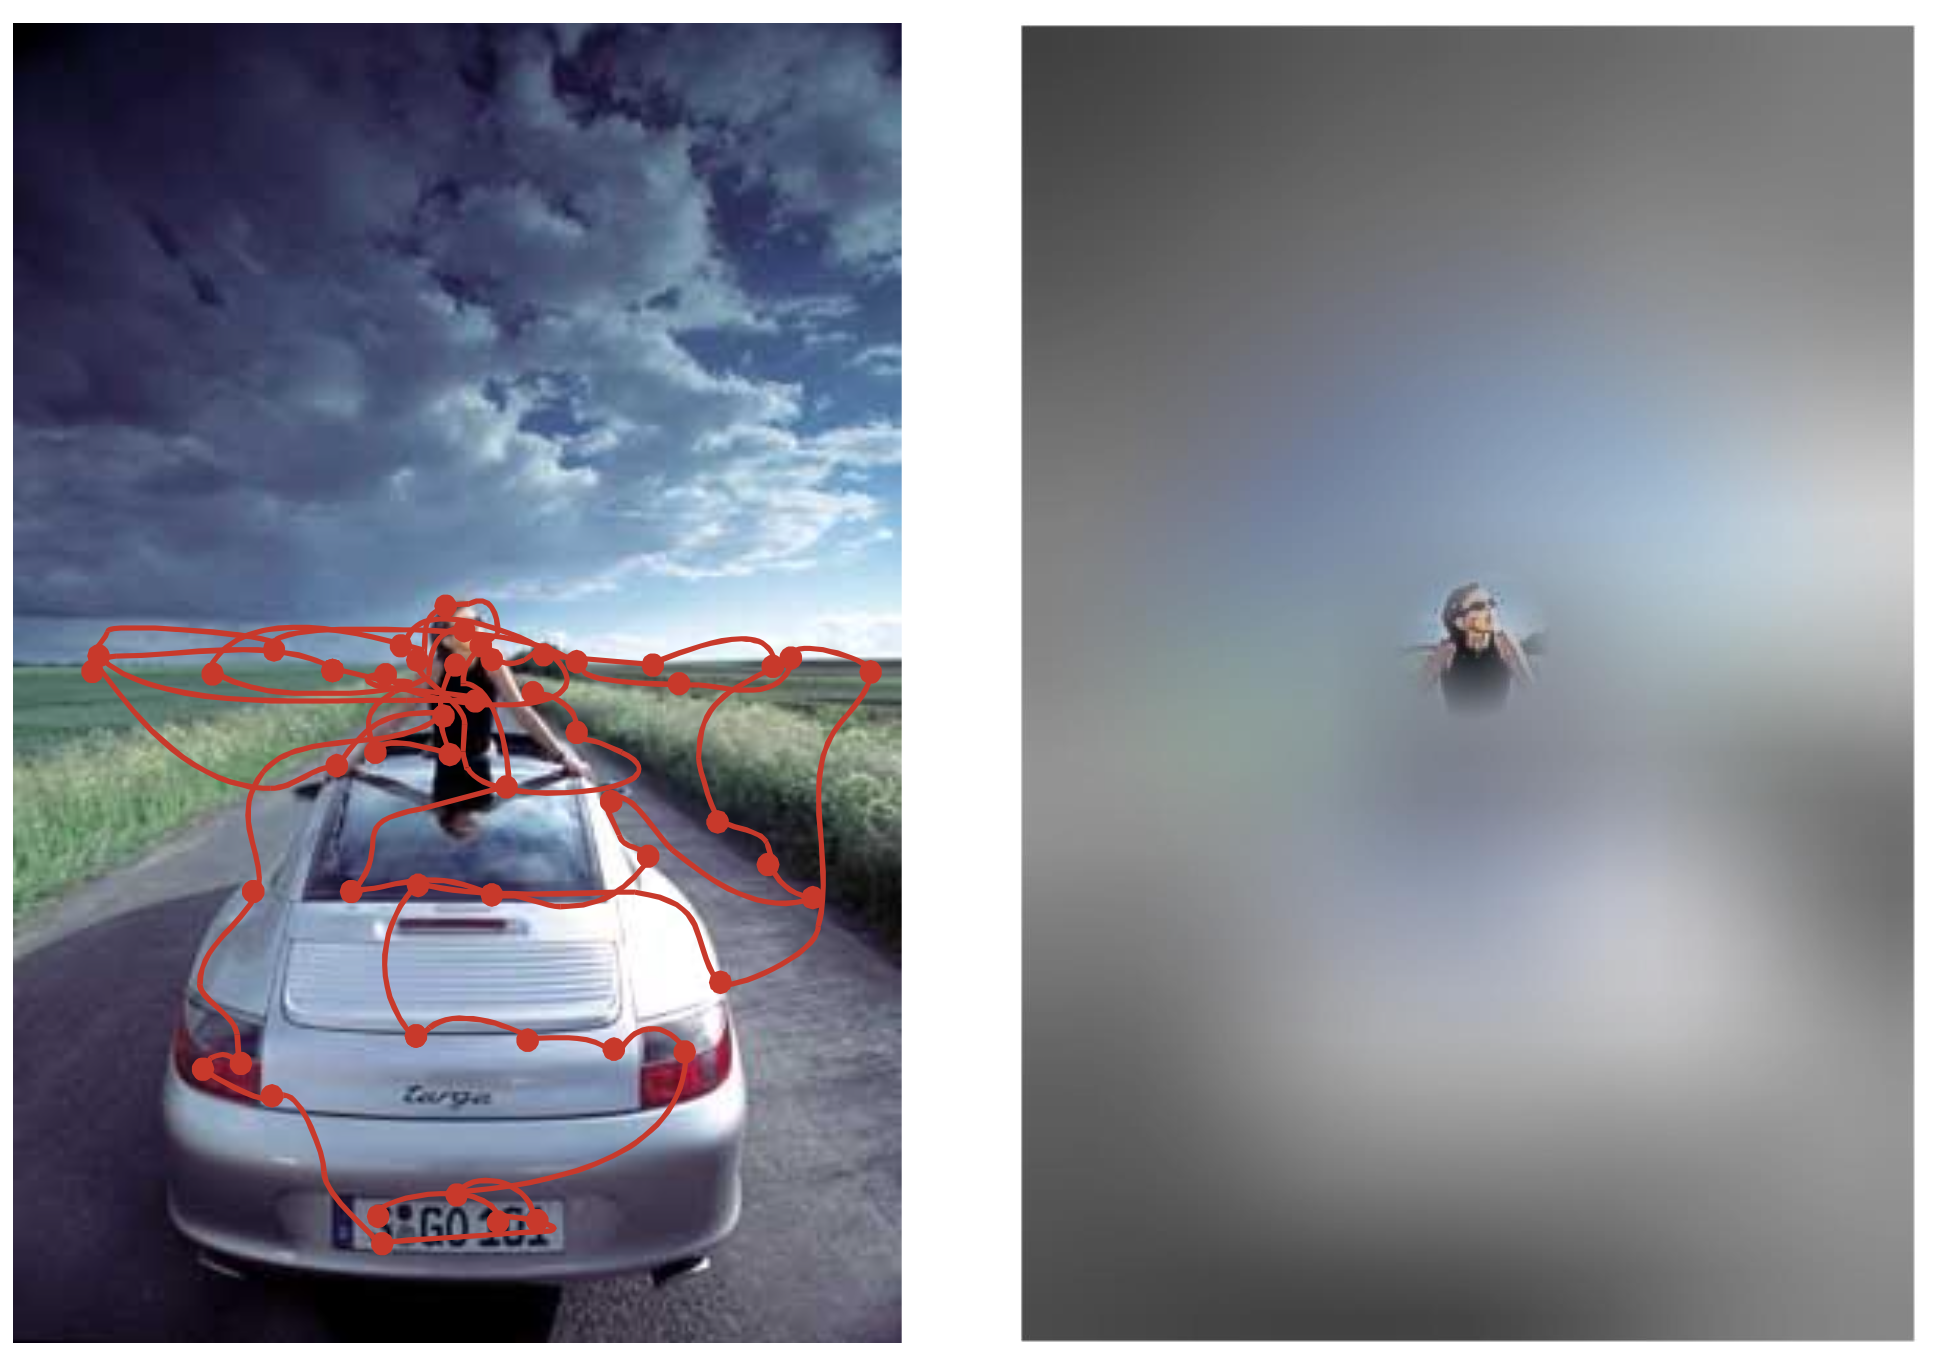
\includegraphics[width=\linewidth]{lec8/figures/fokus.png}
  \end{minipage}
\end{figure}
Organismen nehmen also, was immer an Informationen aus der Umwelt erhältlich ist, bewerten diese auf der Grundlage ihrer Erfahrungen und passen ihre Interpretationsschemata fortlaufend an. Dadurch können sie gut und schnell reagieren. \textbf{Ziel: Regeln für die Informationsintegration in Organismen verstehen!}

\textbf{Was sind Biologische Sinnessysteme?} Umwandlung von physikalischen Reizen aus der Umwelt in Signale des Nervensystems. Bei der \textbf{Sinnesphysiologie} geht es dann um die Untersuchung der Funktion der Sinnessysteme und der Wahrnehmung von äußeren Umweltreizen. Das Pendant hierzu in der Technik sind technische Sensoren und die Messtechnik.
\\\\
Biologische Sinnessysteme haben folgende Eigenschaften:
\begin{itemize}
    \item Sehr hohe Empfindlichkeit
    \item Hohe Toleranz gegenüber Rauschen (hochselektiv)
    \item Reagieren vorwiegend auf Änderungen
    \item Hohe Bandbreite an Komplexität (Einfach – sehr komplex)
    \item Große Bedeutung für das Überleben der Tiere $\rightarrow$ Analyse im Zusammenhang mit Betrachtung der Ökologie
\end{itemize}
Technische Sensoren:
\begin{itemize}
    \item Hohe Empfindlichkeit erfordert erhöhten Energieaufwand und erhöhtes Gewicht
    \item Häufig sehr komplex
    \item Messung von absoluten Werten
\end{itemize}
\textcolor{red}{
\textbf{Ziele der bionischen Sensorik:}
\begin{itemize}
    \item Optimierung von technischen Sensoren
    \item Konstruktion neuartiger Sensoren nach dem
Vorbild der Natur
\end{itemize}
}

\subsubsection{Grundlegende Organisation von Nervensystemen}

Der Aufbau des Nervensystems ist wie im folgenden Bild beschrieben. Zentralnervensysteme (ZNS) sind Ansammlungen von Nervenzellen, wobei solche Ansammlungen am vorderen Pol eines Tieres auch \textbf{Gehirne} genannt werden. Gehirne werden unterteilt in:
\begin{itemize}
    \item \textbf{Ganglion:} normale periphere Zellmasse, manchmal auch zentral: Basalganglien. In den Ganglien finden sich die Zellkörper (Somata) der Nervenzellen.
    \item \textbf{Nucleus:} mehrere Zellkörper zusammen, im ZNS gelegen, oft gut abgrenzbar vom restlichen Gewebe.
    \item \textbf{Markstrang:} Strangartige Anordnung von NZ und Axonen, keine Sonderung in Ganglien und Nerven, bei einigen Wirbellosen $\rightarrow$ z.B.\ Quallen
\end{itemize}

\begin{center}
    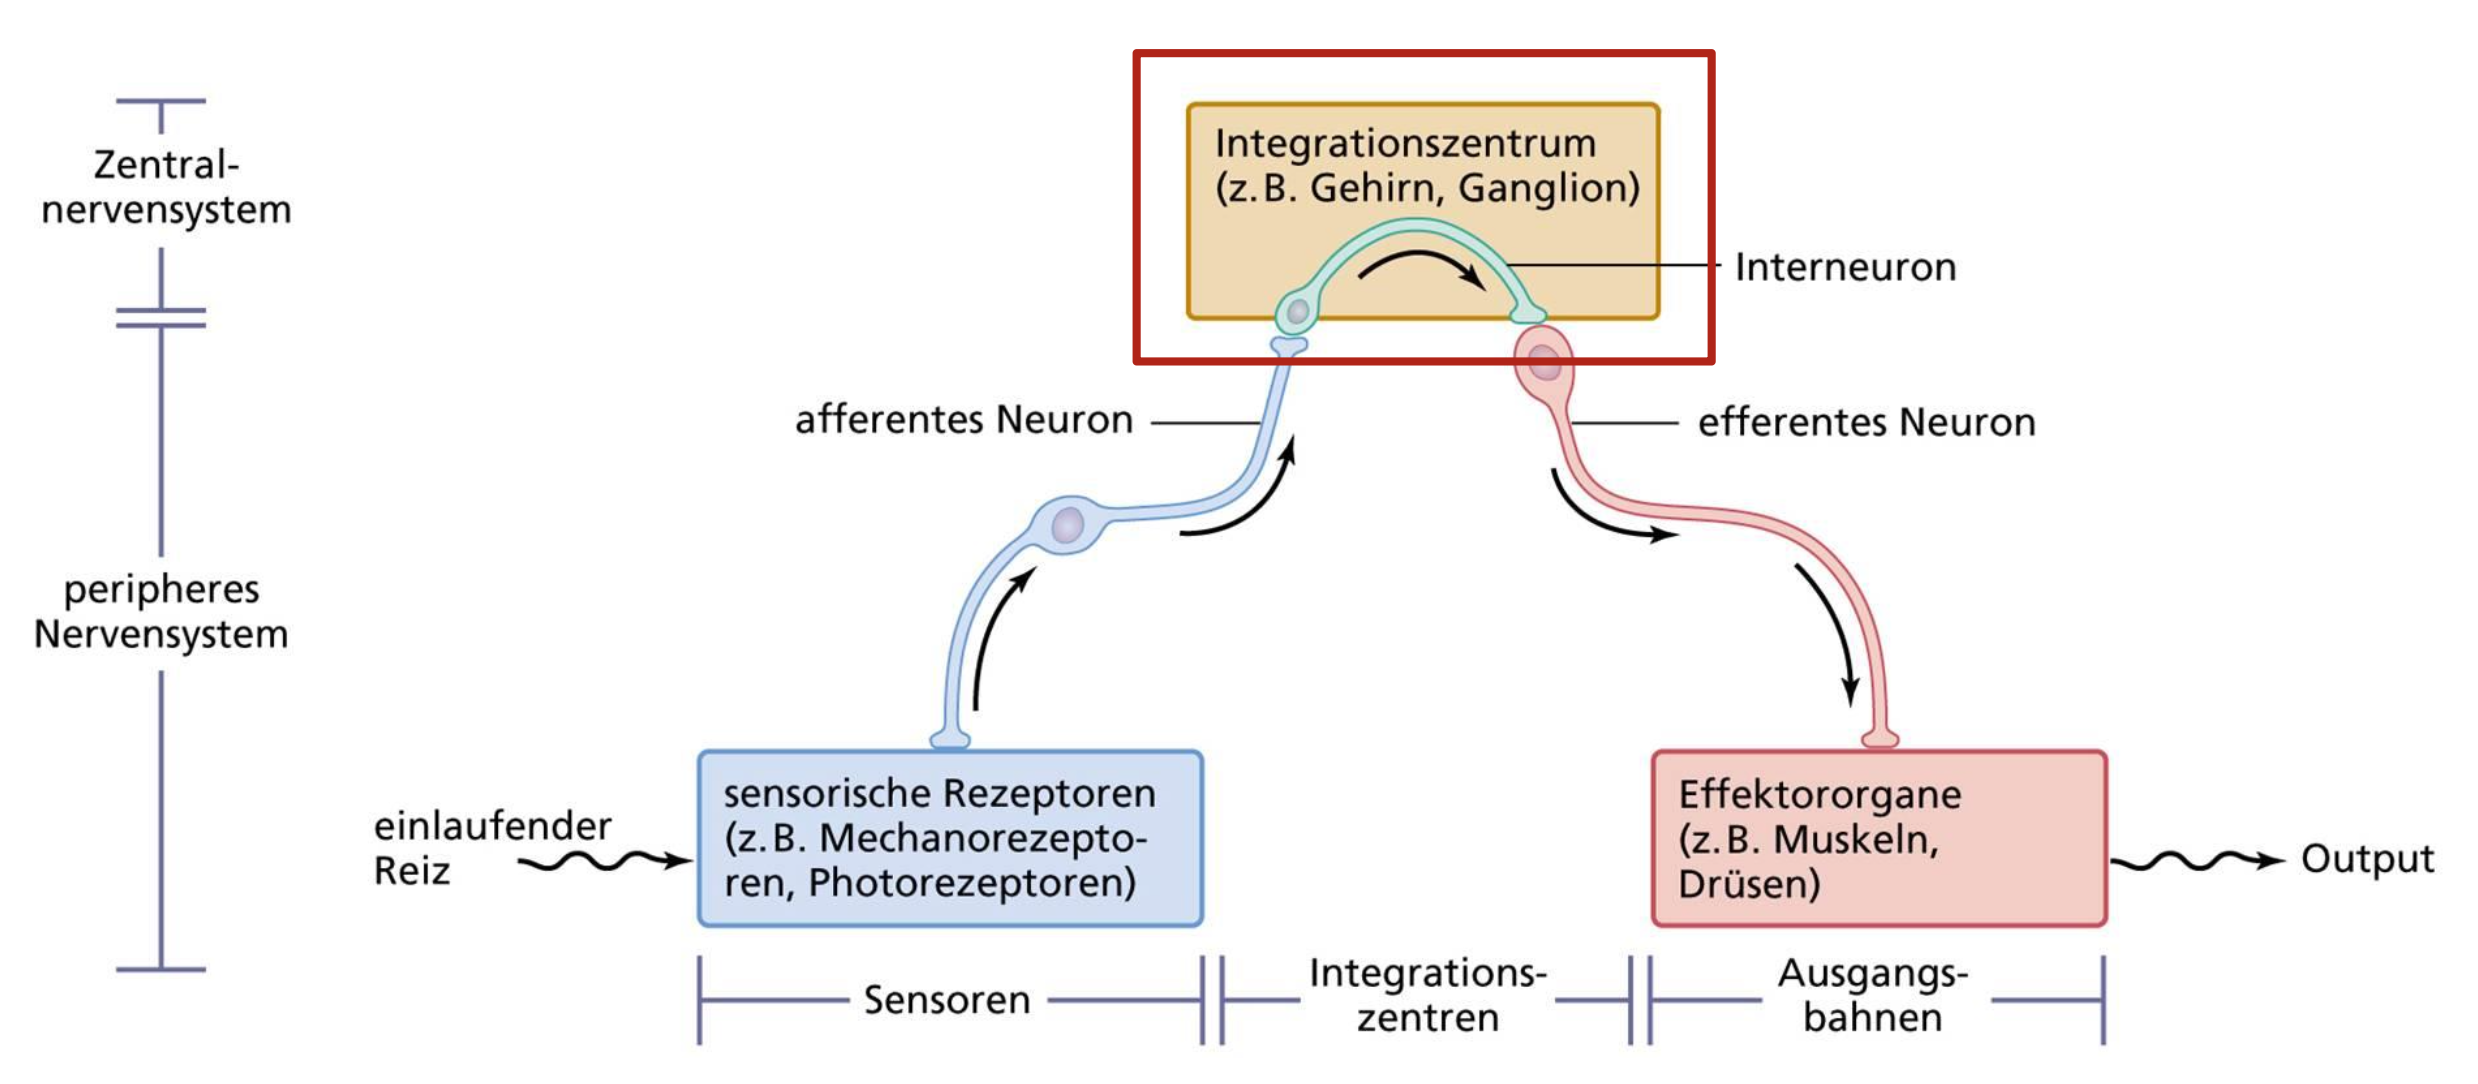
\includegraphics[width=16cm]{lec8/figures/nervensystem.png}
\end{center}
Bei Wirbeltieren ist ein Gehirn mit verschiedenen Unterbereichen ausgeprägt.

\subsubsection{Sensoren und Sinnessysteme}

Es gibt 5 Sensortypen \dangersign:
\begin{itemize}
    \item Mechanosensoren: Haut, Muskel, Ohr, Gleichgewichtsorgan, Seitenlinie
    \item Temperatursensoren: Haut, Infrarotsinn
    \item Chemosensoren: Geschmack, Geruch, CO2-Rezeptoren
    \item Photorezeptoren: Stäbchen und Zapfen der Retina
    \item Nozisensoren: registrieren Gewebeschädigungen
\end{itemize}
Viele Sensoren vom gleichen Typ bilden ein Sinnesorgan. Um die Nervenzellaktivität aufzuzeichen gibt es 4 Möglichkeiten.
\begin{itemize}
    \item extra / -intrazelluläre Ableitung (Elektrode in der Nähe der Nervenzelle platzieren; im Bild oben links)
    \item patch-clamp (Einzelne Kanäle ``einsaugen''; im Bild unten links)
    \item Voltage-sensitive dyes (Einfärben der Nervenzellen; im Bild oben rechts)
    \item Magnet-Resonaz-Imaging (MRI) $\rightarrow$ hier entstehen auch statistische Fehler
\end{itemize}

\begin{center}
    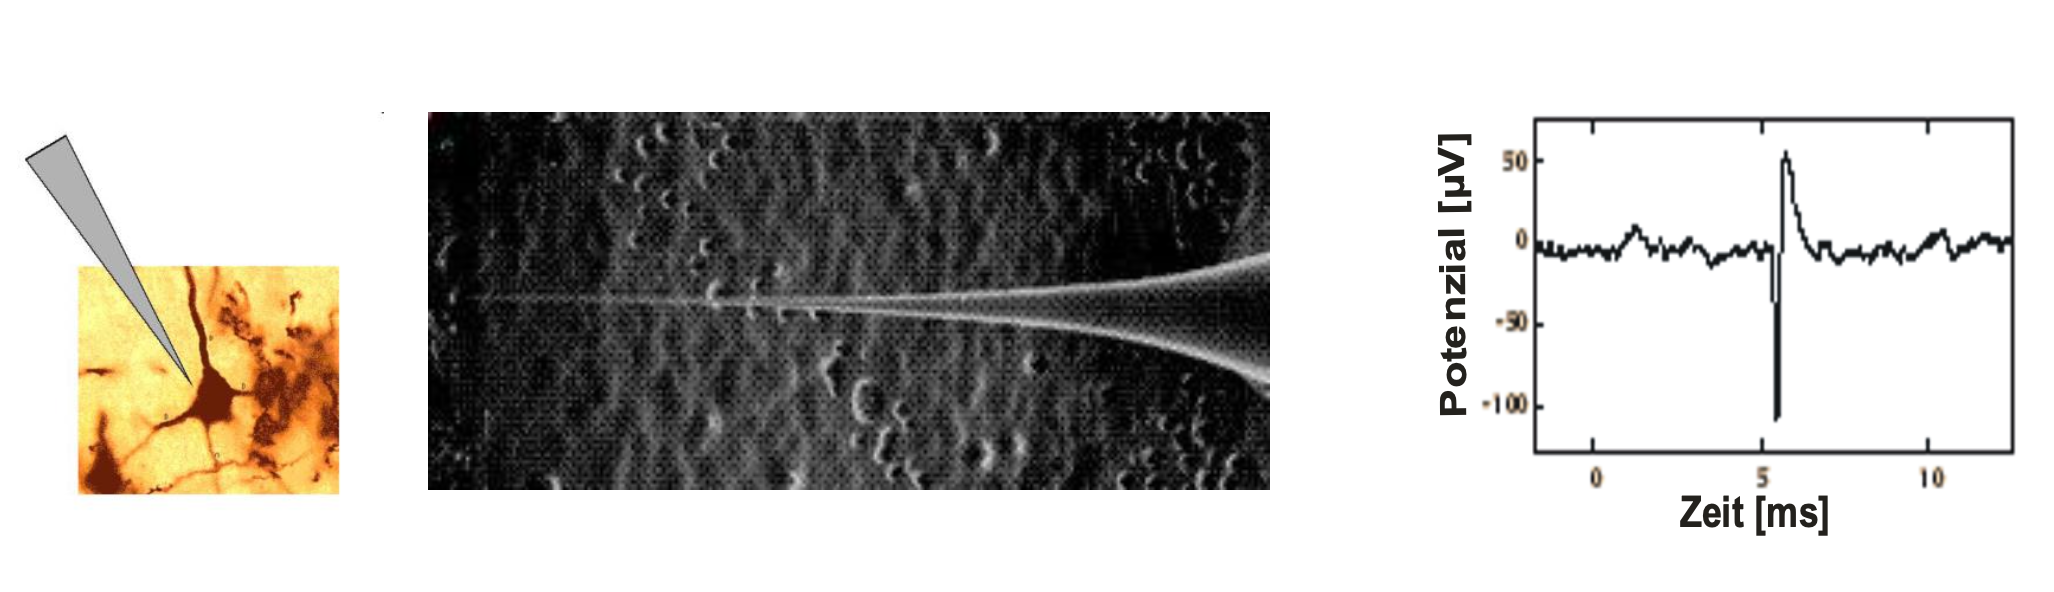
\includegraphics[width=10cm]{lec8/figures/elektrode.png}
    \hfill
    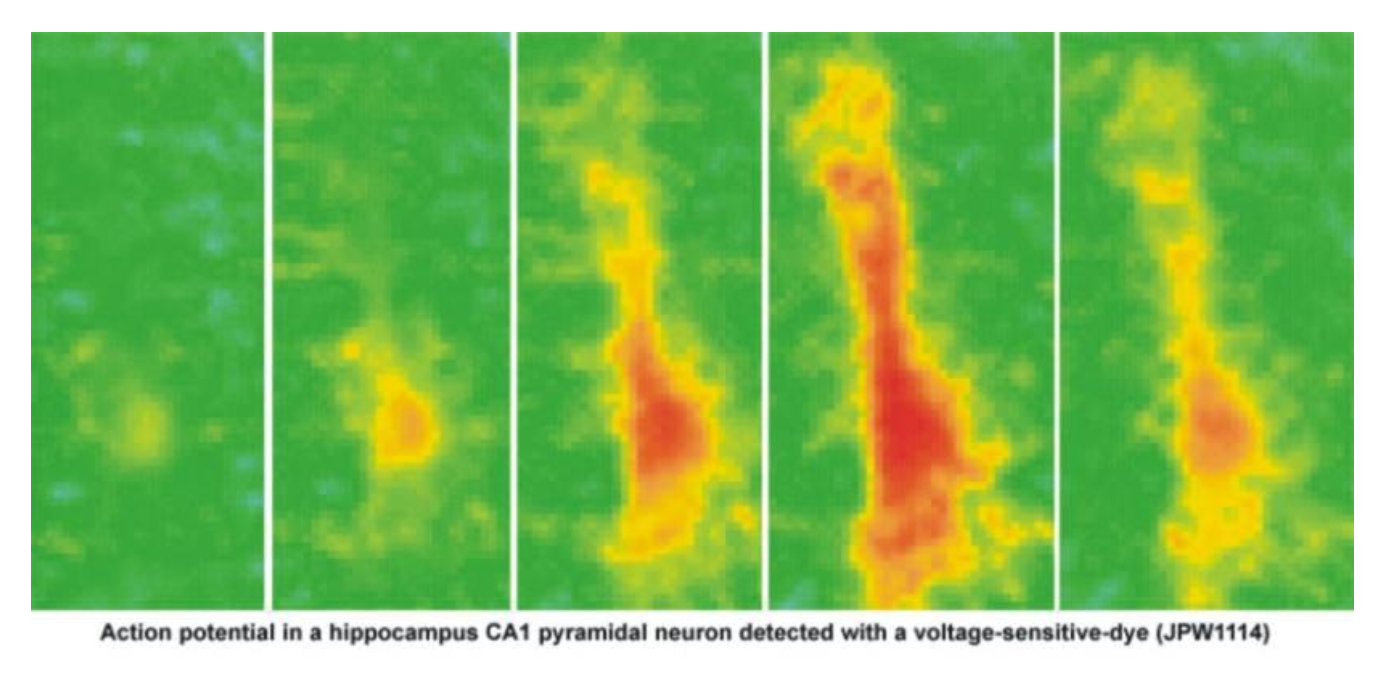
\includegraphics[width=6cm]{lec8/figures/dye.png}
    \\
    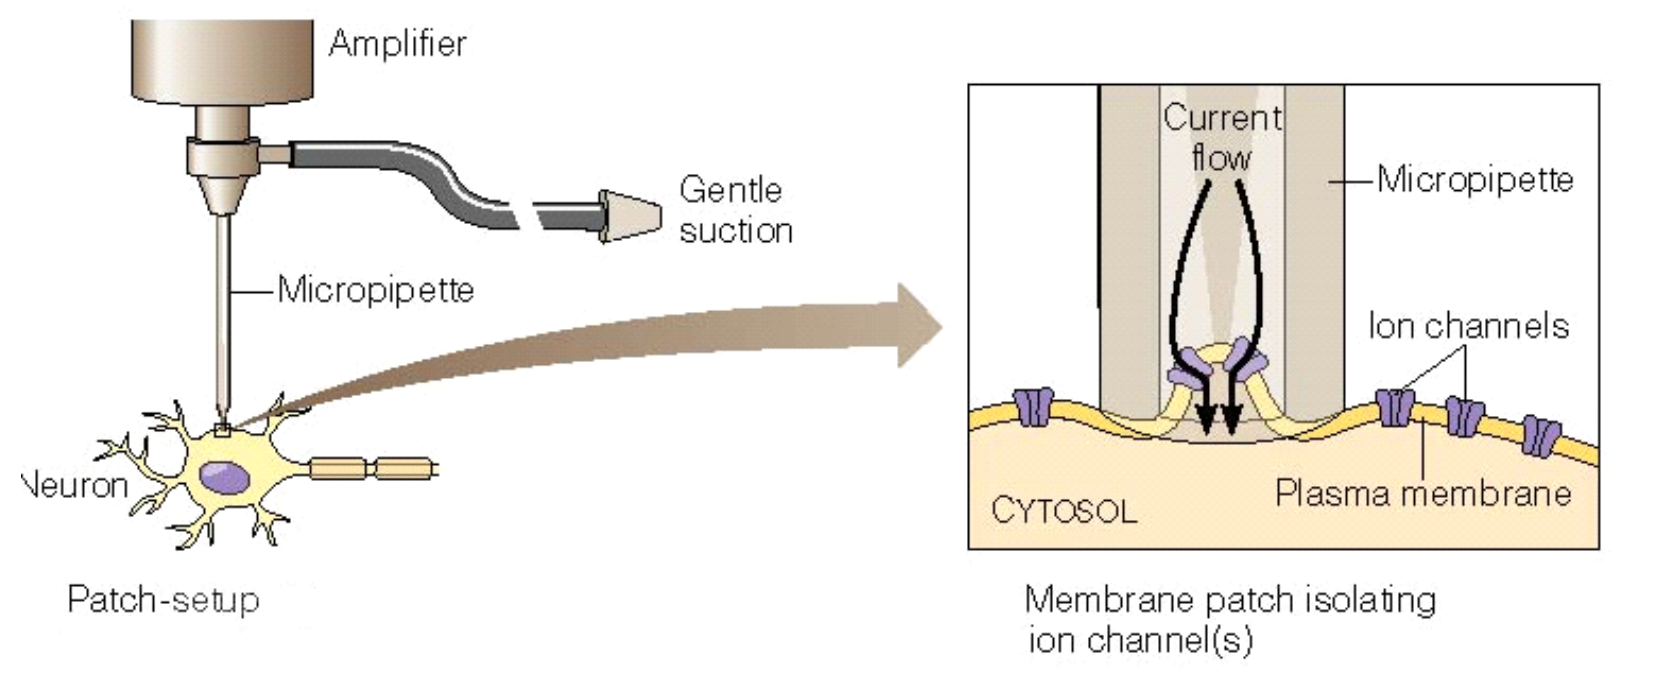
\includegraphics[width=10cm]{lec8/figures/clamp.png}
    \hfill
    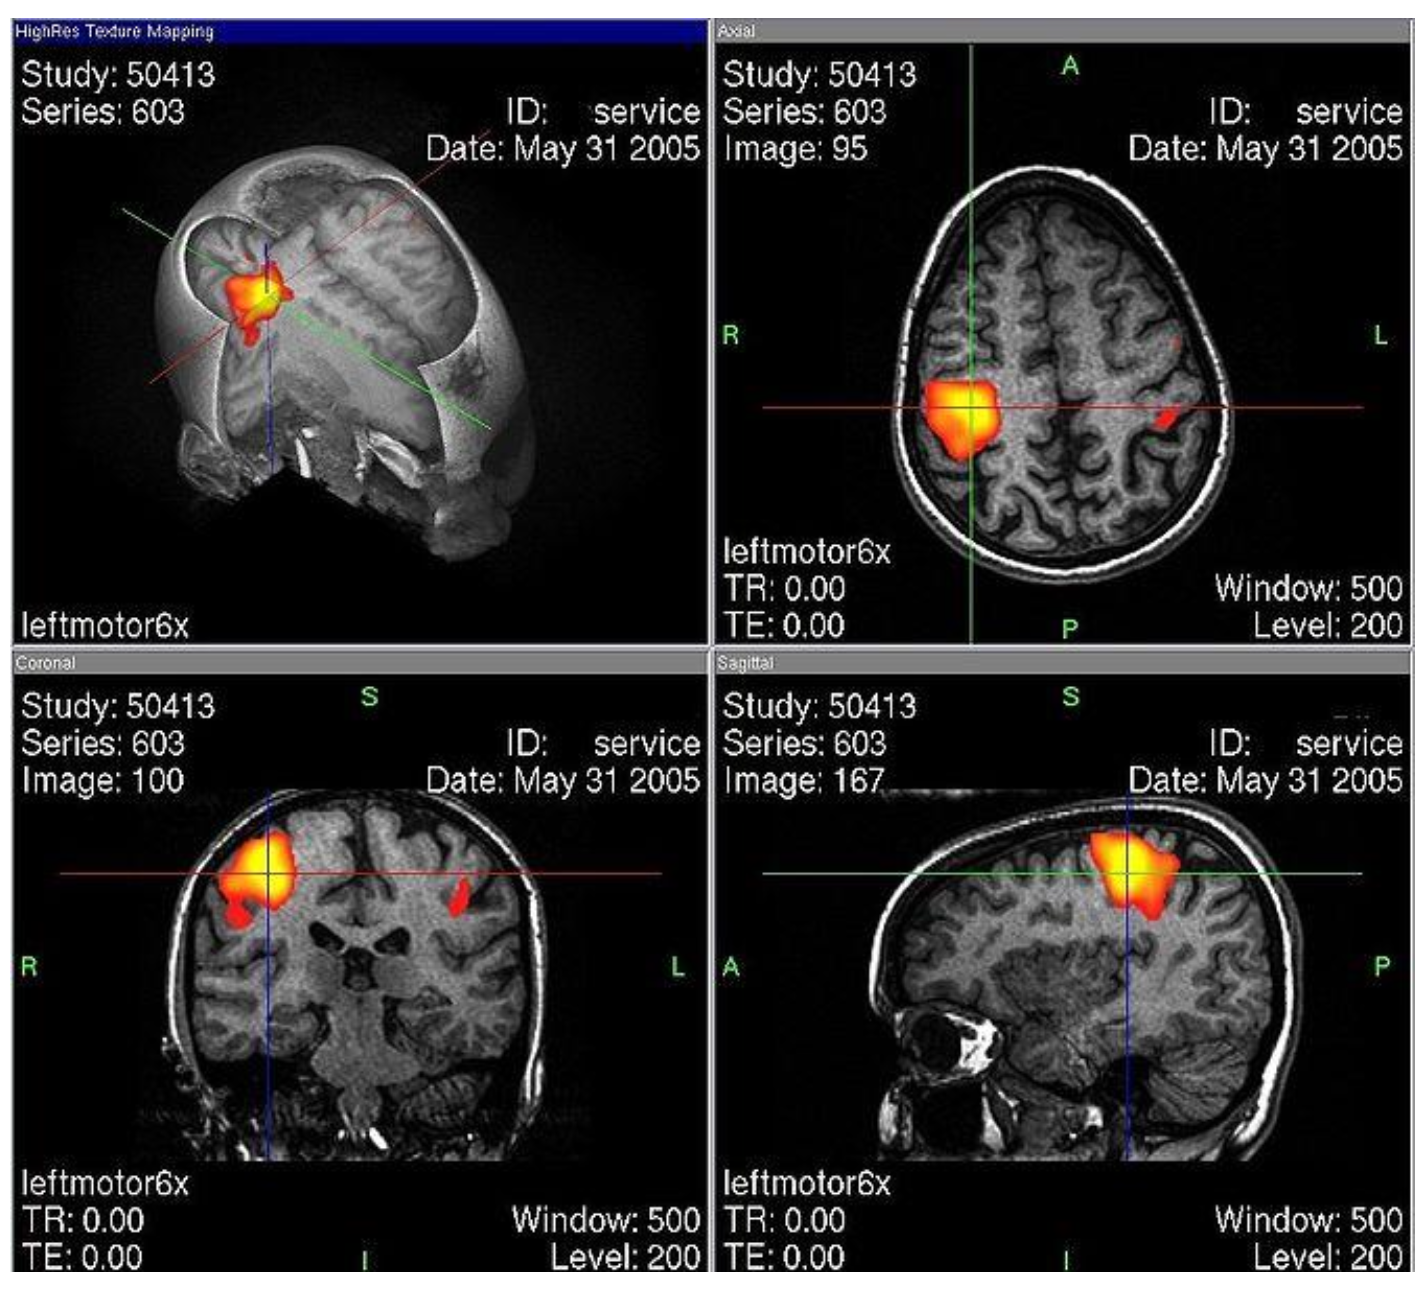
\includegraphics[width=6cm]{lec8/figures/MRI.png}
\end{center}

\subsubsection{Infrarotwahrnehmung von Schlangen}

Manche Schlangenarten besitzen ein Sinnesorgan, um per Infrarotwahrnehmung Beute zu lokalisieren (auch im Dunkeln), Feinde zu erkennen und Aufwärmplätze zu finden. In den nachfolgenden Infrarotbildern ist zu erkennen, dass der Kontrast der Beutetiere zum Hintergrund ausreichend ist, um es gezielt anzugreifen. Nordamerikanische Erdhhörnchen haben sich durch Coevolution an Schlangen mit Infrarotwahrnehmung angepasst, indem sie die Blutzufuhr in ihren Schwanz regulieren,  damit seine Temperatur anpassen und anschließend mit dem Schwanz wedeln, um die Schlangen zu irritieren.
\\\\
Warmblütige Tiere emittieren bei ca.\ 310 Kelvin IR-Strahlung mit eine Wellenlänge von $10\mu m$. Die Sinneswahrnehmung der Schlange demnach auf einen Bereich $0,75 \mu m \leq \lambda \leq 15 \mu m$ optimiert.
\\\\
\textbf{Biologische IR-Sensoren sind (meistens) Bolometer und funktionieren nach dem Prinzip \dangersign:} \textcolor{red}{IR-Strahlung trifft ein $\rightarrow$ Absorption in wasser- und bluthaltigem Gewebe $\rightarrow$ Wärme- und Temperatur-Zunahme auf der Grubenmembran $\rightarrow$ Wahrnehmung durch Temperaturrezeptoren}. Dazu sind biologische Bolometer effiziente Absorber, die Grubenmenbran hat eine geringe thermische Masse und ist gut gegen den Körper isoliert (durch eine luftgefüllte Kammer). Im nachfolgenden Bild rechts ist ein biologisches Bolometer angebildet, welches zusätzlich noch ein ``Lochkameraprinzip'' verwendet. Bei Schlangen produziert das Bolometer ein unscharfes Bild, da es wenige Rezeptoren dort gibt, wobei es Indizien gibt, dass das Bild neuronal nachgeschärft wird.

\begin{center}
    \includegraphics[width=6cm]{lec8/figures/wärmebild.png}
    \hfill
    \includegraphics[width=3.5cm]{lec8/figures/erdhörnchen.png}
    \hfill
    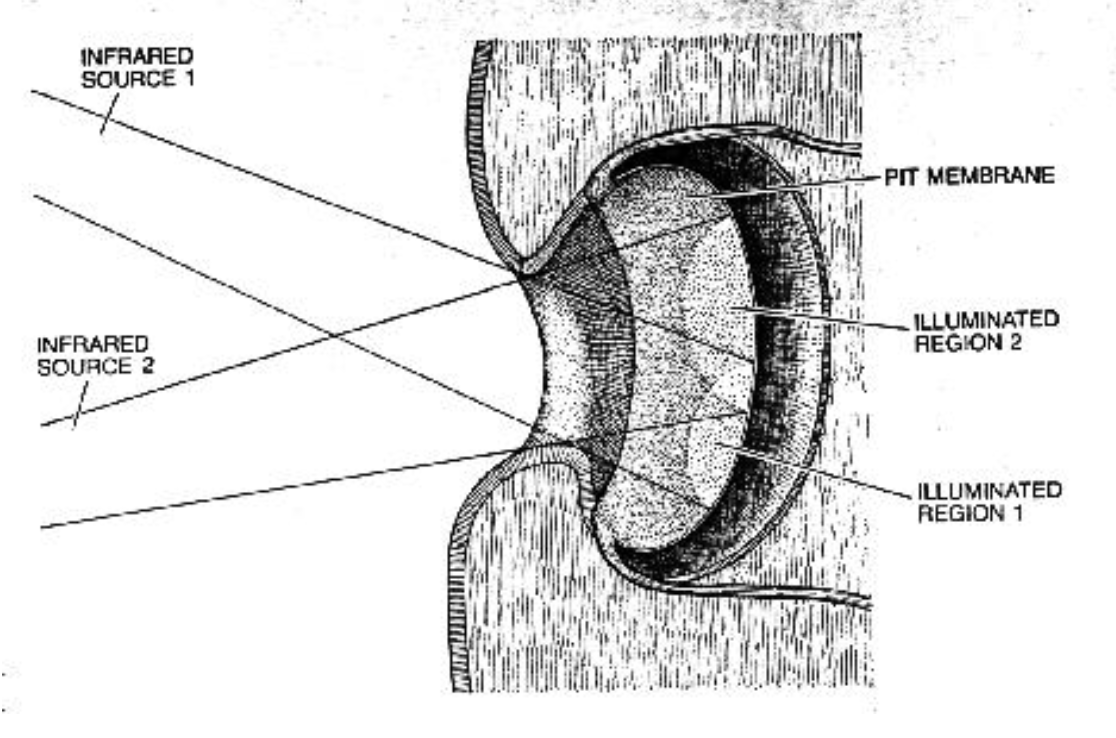
\includegraphics[width=6.5cm]{lec8/figures/bolometer.png}
\end{center}

Die Schlange überlagert die Signale aus dem visuellen Wahrnehmungssinn und der IR-Wahrnehmung in bimodalen Neuronen.

\begin{center}
    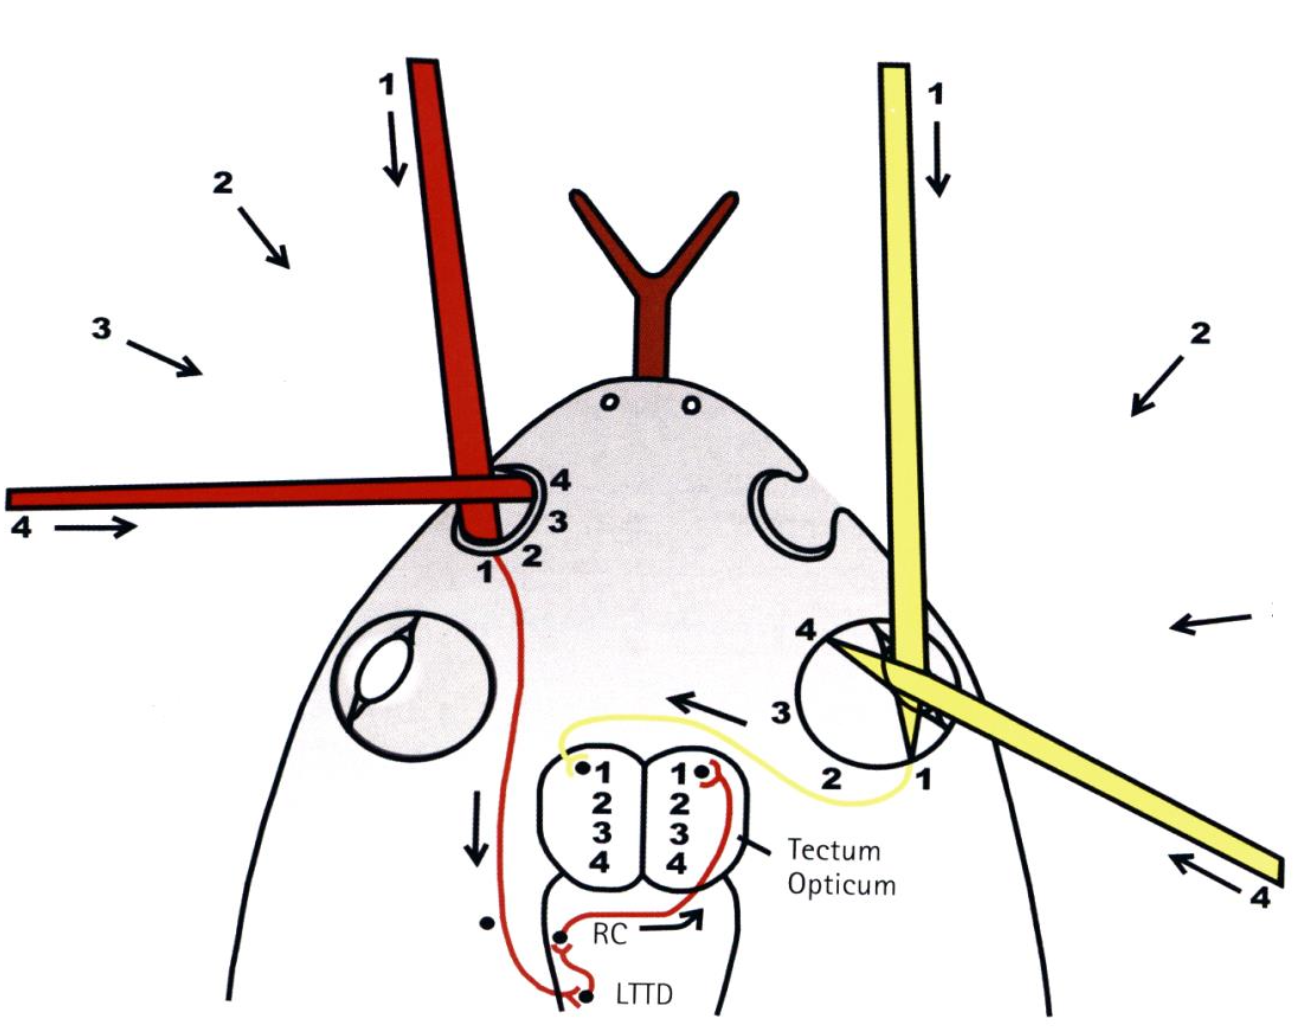
\includegraphics[width=8cm]{lec8/figures/sinne.png}
    \hfill
    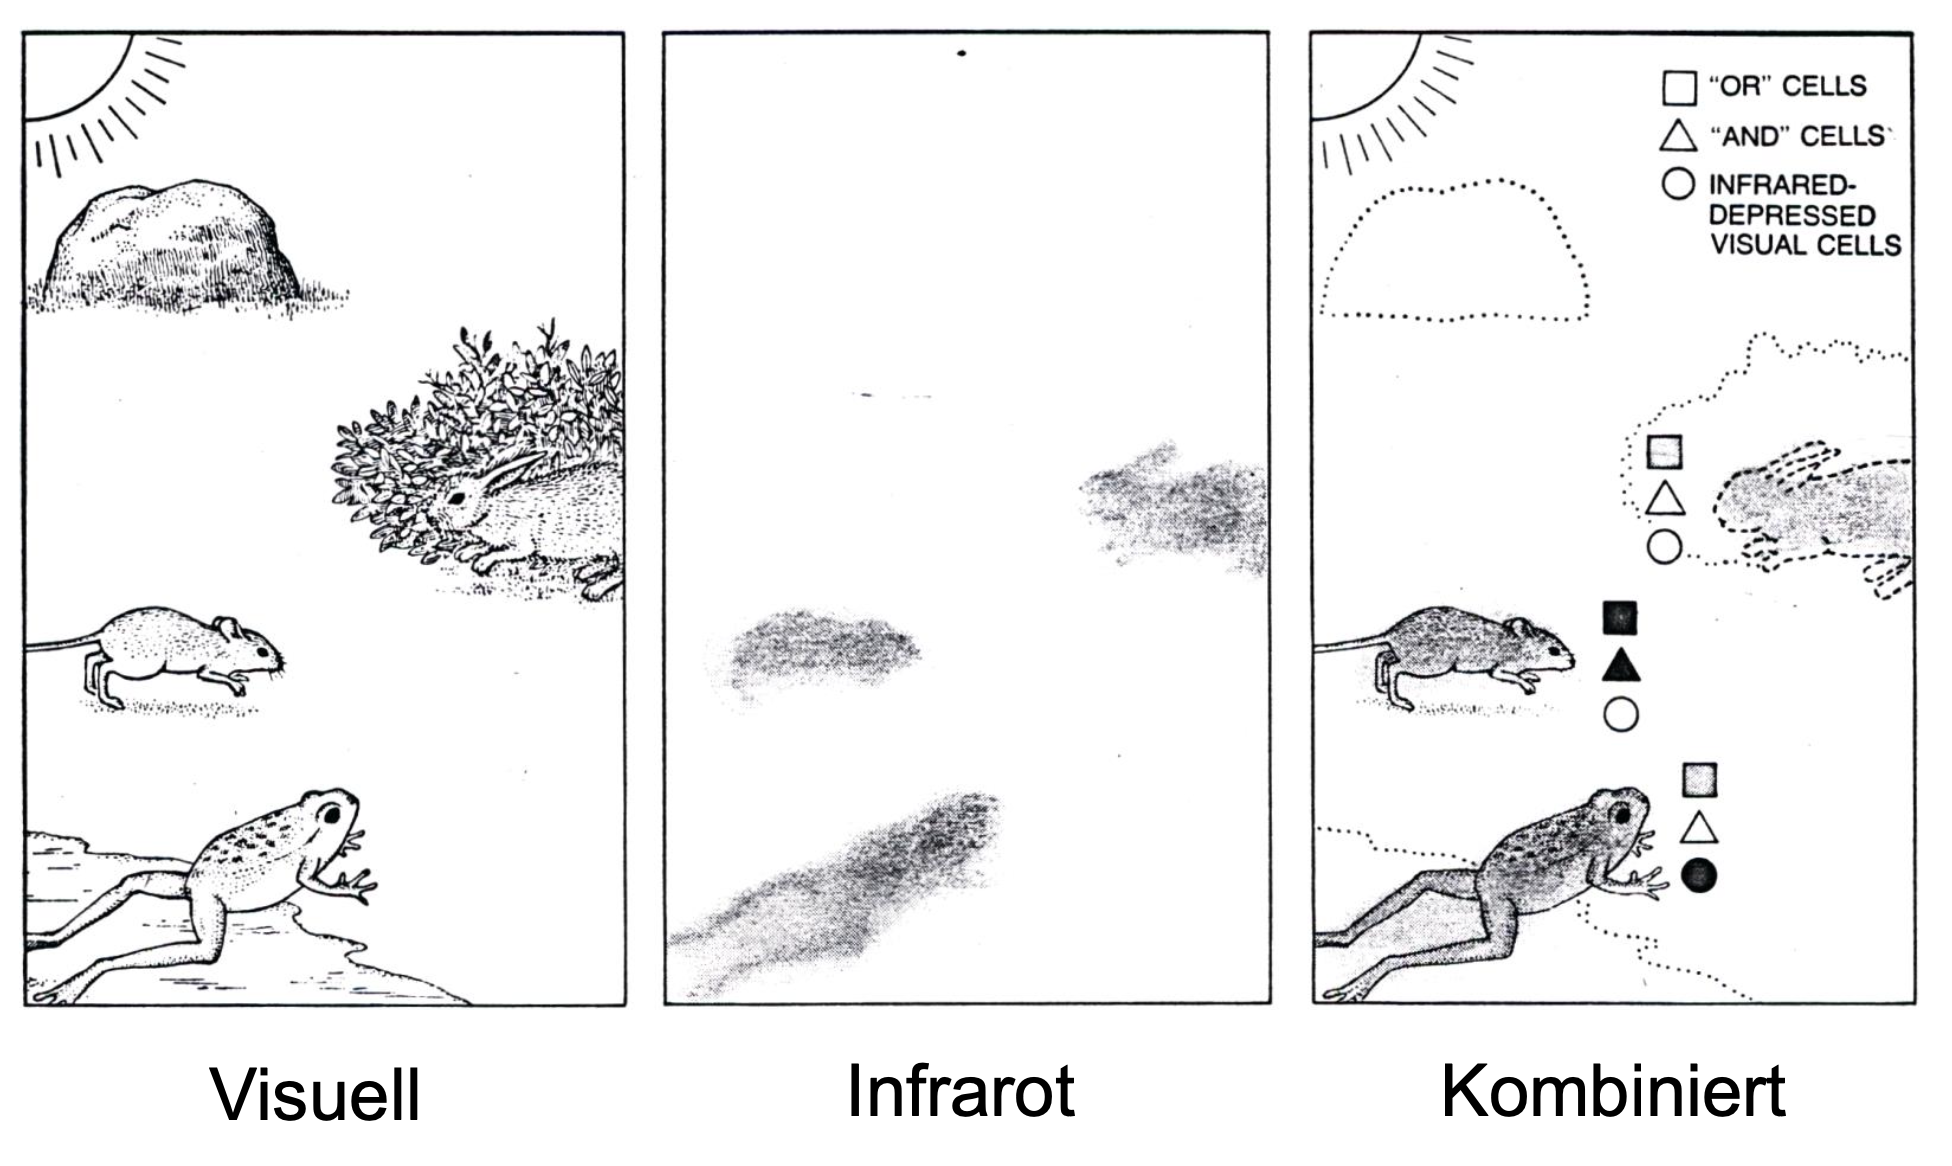
\includegraphics[width=8cm]{lec8/figures/kombiniert.png}
\end{center}
 
 \subsubsection{Weitere Infrarotsensoren im Tierreich}

\paragraph{Vampirfledermäuse} Diese Fledermäuse besitzen Infrarotsensoren in der Nasenregion, wobei deren Transduktionsmechanismus vergleichbar mit dem von Schlangen ist. 

\paragraph{Feuerkäfer} Sie fliegen gezielt Waldbrände an (Orientierung durch Geruch, IR?), paaren sich im Waldbrandgebiet und legen ihre Eier in geschädigten Bäumen (Abwehrmechanismen stark geschwächt) ab. Dabei dienen die Infrarotsensoren auch zum Auffinden von bereits abgekühlten Flächen. Die Infrarotsensoren unterscheiden sich zwischen den pyrophilen Käfern. Während manche den Bolometern der Schlangen ähneln (siehe im Bild oben links; Acanthocnemus), bedienen sich andere an einem ``photo-mechanischen'' Transduktionsprinzip \dangersign (siehe im Bild unten links). Hierbei wird die Ausdehnung einer Flüssigkeit durch Temperaturerhöhung genutzt, um Signale an Druckrezeptoren zu aktivieren.

\textbf{Bionische Anwendung des ``photo-mechanischen'' IR-Sensors \dangersign:} Dabei erwärmt die einkommende IR-Strahlung Wasser in der Druckkammer, wodurch sich das Flüssigkeitsvolumen erhöht und einen Kondensator auslenkt. Die Spannungsänderung am Kondensator infolge der Auslenkung kann dann gemessen werden. 

\textit{Mögliche Klausurfrage: Erklären sie das Funktionsprinzip des bionischen Vorbildes und der technischen Anwendung.} 

\begin{center}
    \includegraphics[width=5cm]{lec8/figures/feuerkäfer.png}
    \hfill
    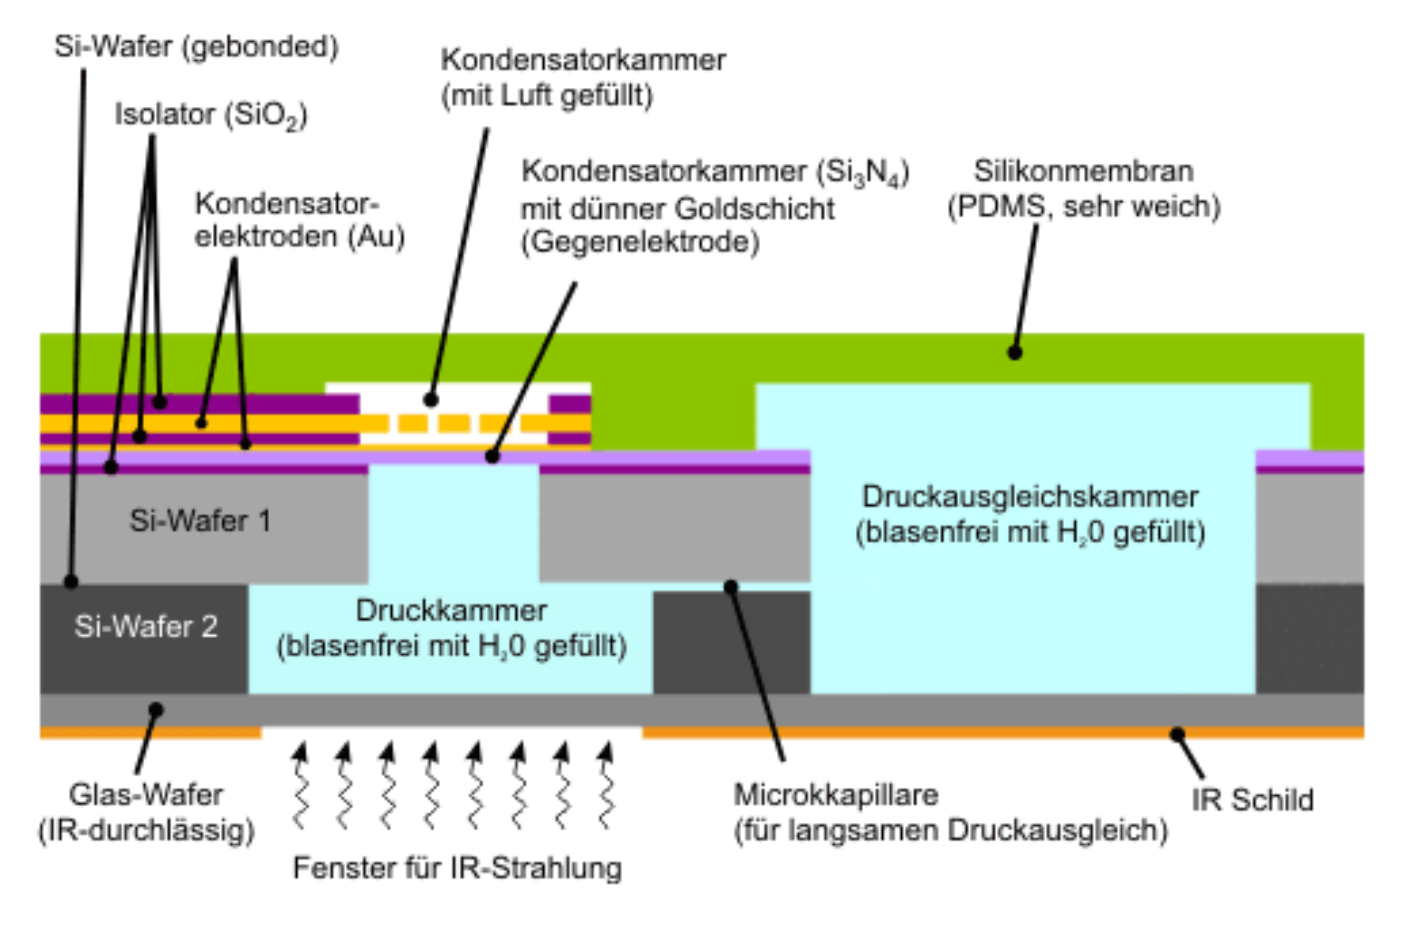
\includegraphics[width=10cm]{lec8/figures/photo-mechanisch-bionisch.png}
    \\
    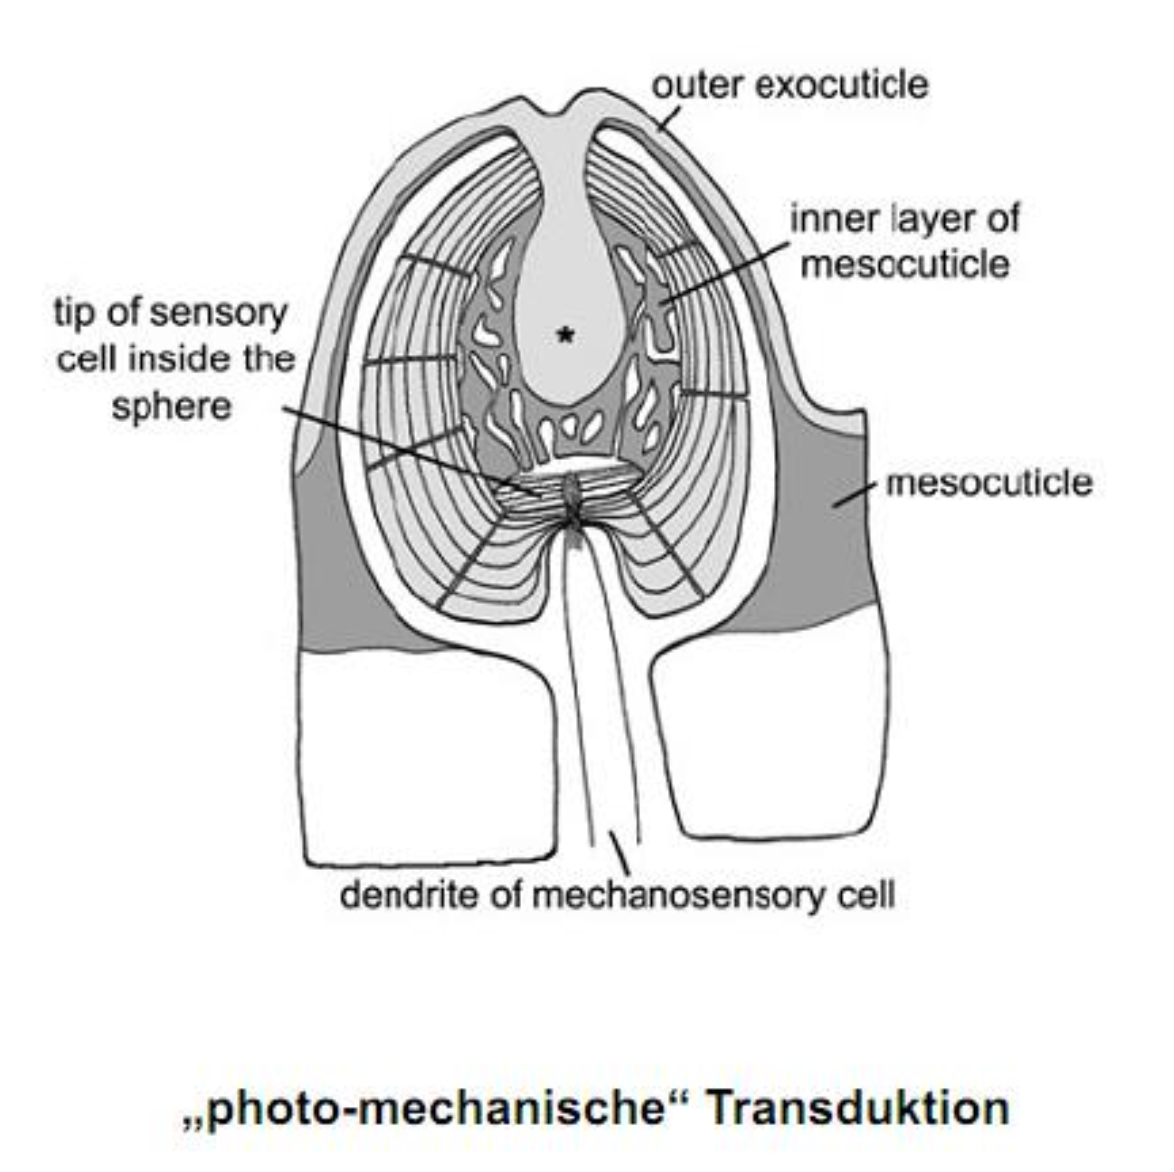
\includegraphics[width=6cm]{lec8/figures/photo-mechanisch.png}
    \hfill
    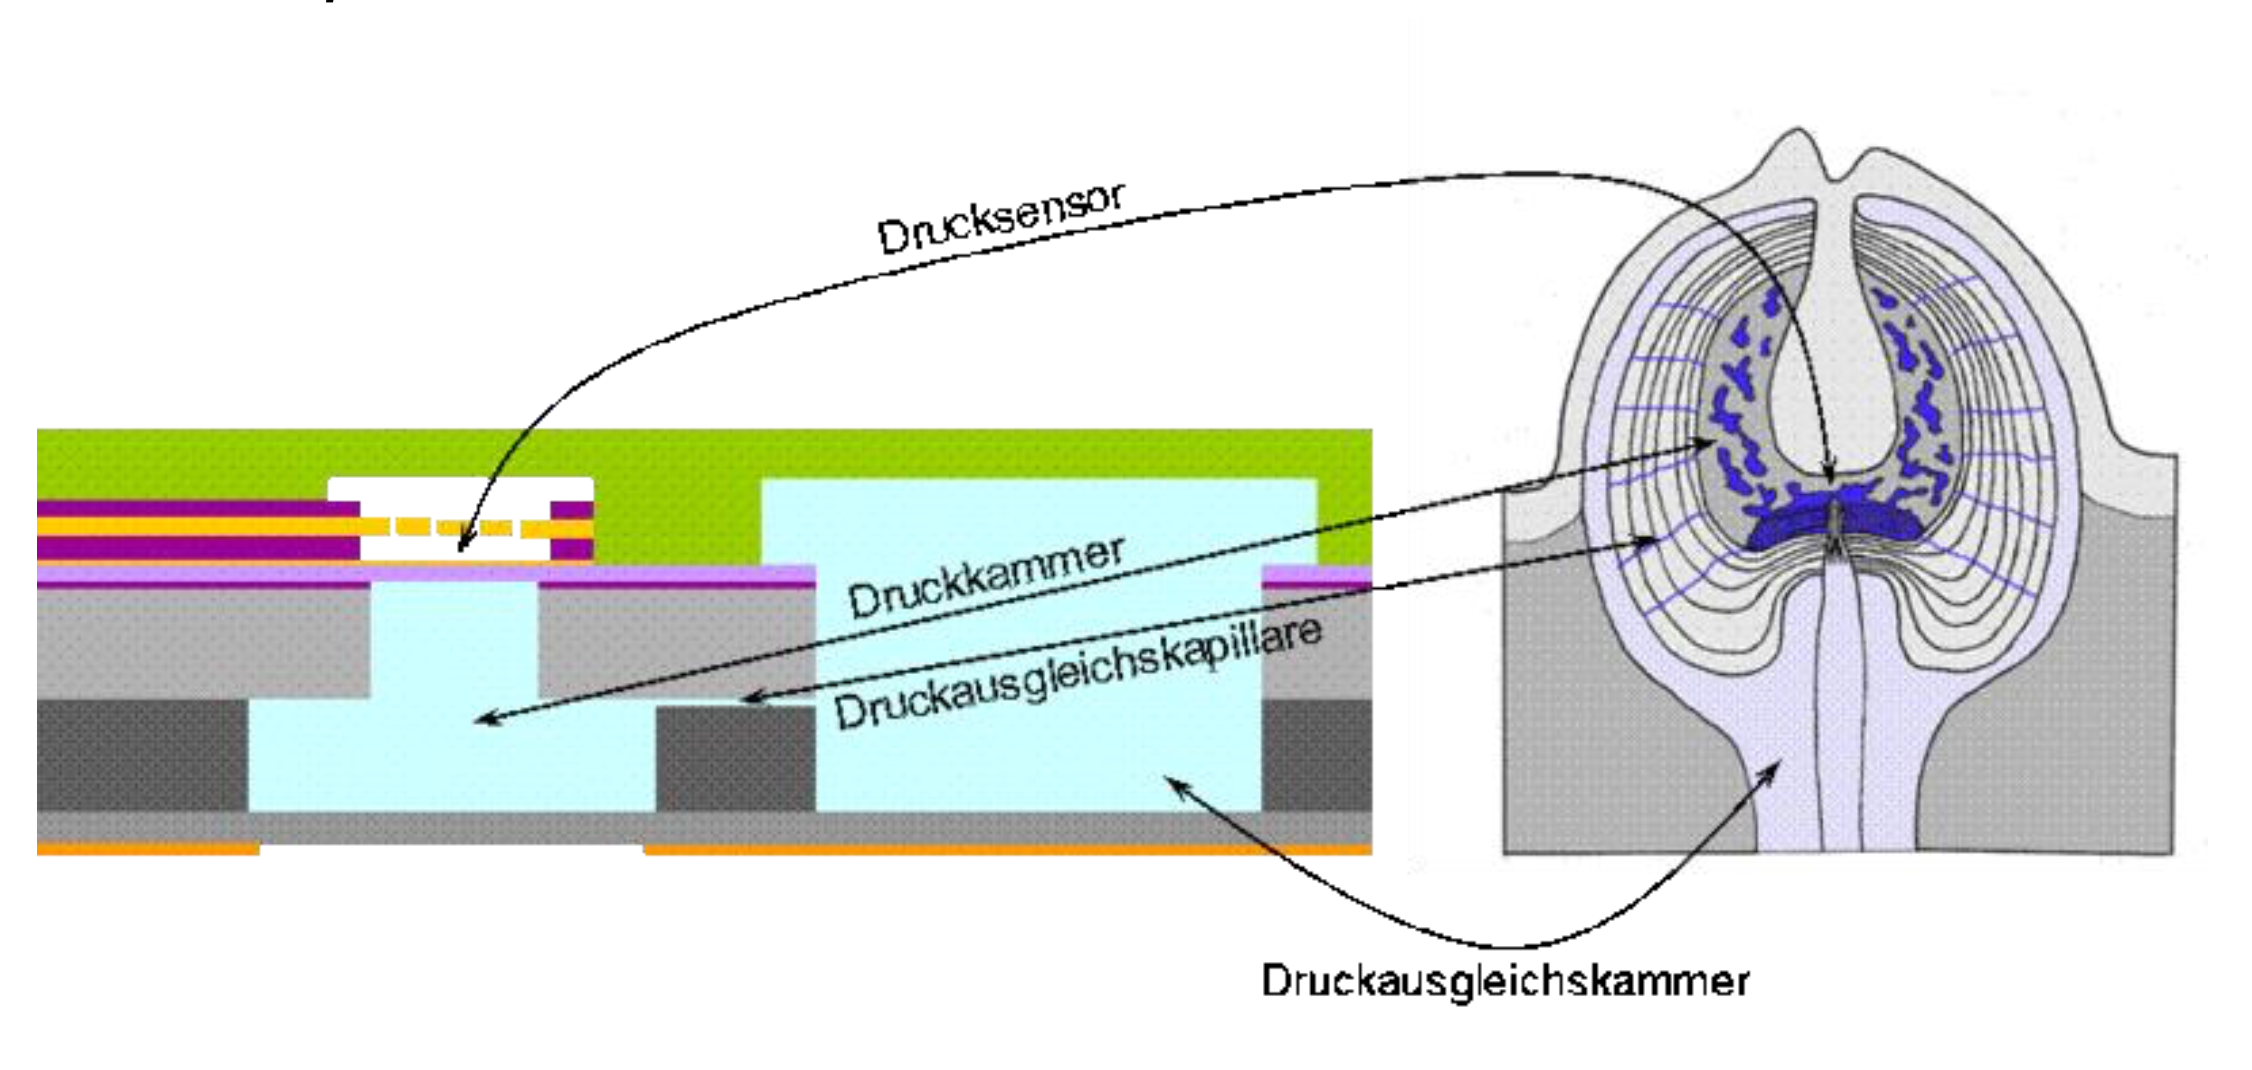
\includegraphics[width=10cm]{lec8/figures/photo-mechanisch-bionisch-2.png}
\end{center}

\subsubsection{Andere Sensorik im Tierreich}

\paragraph{Seitenliniensystem der Fische \dangersign} Bewegungen von Objekten führen zu Wasserschwingung, welche durch das Seitenlinienorgan wahrgenommen werden können. Dabei werden Sensoren durch mechanosensitve Elemente gebildet. Die Seitenlinien sind in (teilweise) dunkel pigmentierte Kanäle an der Fischseite und am Kopf eingelassen und bestehen aus \textbf{zwei Grundelementen: freie Neuromasten} (an der Schuppenoberfläche) und \textbf{Kanalneuromasten} (unter den Schuppen je zwischen zwei Kanalöffnungen). Die \textit{freien Neuromasten codieren die Geschwindigkeit der Wasserbewegungen}, während die \textit{Kanalneuromasten die Beschleunigung der Wasserteilchen zwischen den Kanalöffnungen codieren} und das Signal an den Seitenliniennerv weitergeben. Bei Fischen in turbulenten Gewässern sind daher vor allem die Kanalneuromasten ausgeprägt.

Wasserbeweguneng von großen Räubern lösen einen Fluchtreflex aus. Die Empfindlichkeit wird mit zunehmender Entfernung zum Objekt durch die Abschwächung der Wasserbewegung drastisch verringert.
\\\\
\textit{Bionische Anwendung des Seitenlinienorgans} \dangersign: Ein bionischer Mechanirezeptor (im Bild unten) bestehte aus einer optischen Faser aus Silikon, einer IR-Diode und einem Fototransistor. Die Strahlung der IR-Diode wird über die Faser in Richtung des Fotortransistors durch den flüssigkeitdurchströmten Kanal geschickt. Wird die Faser durch die Strömung ausgelenkt, so wird das Signal unterbrochen, was messtechnisch erfasst wird. Das künstliche Seitenlinienorgan besteht letztendlich aus einer Batterie dieser Mechanirezeptoren und ist in der Lage Wassergeschwindigkeiten/Durchfluss zu messen.

\begin{center}
    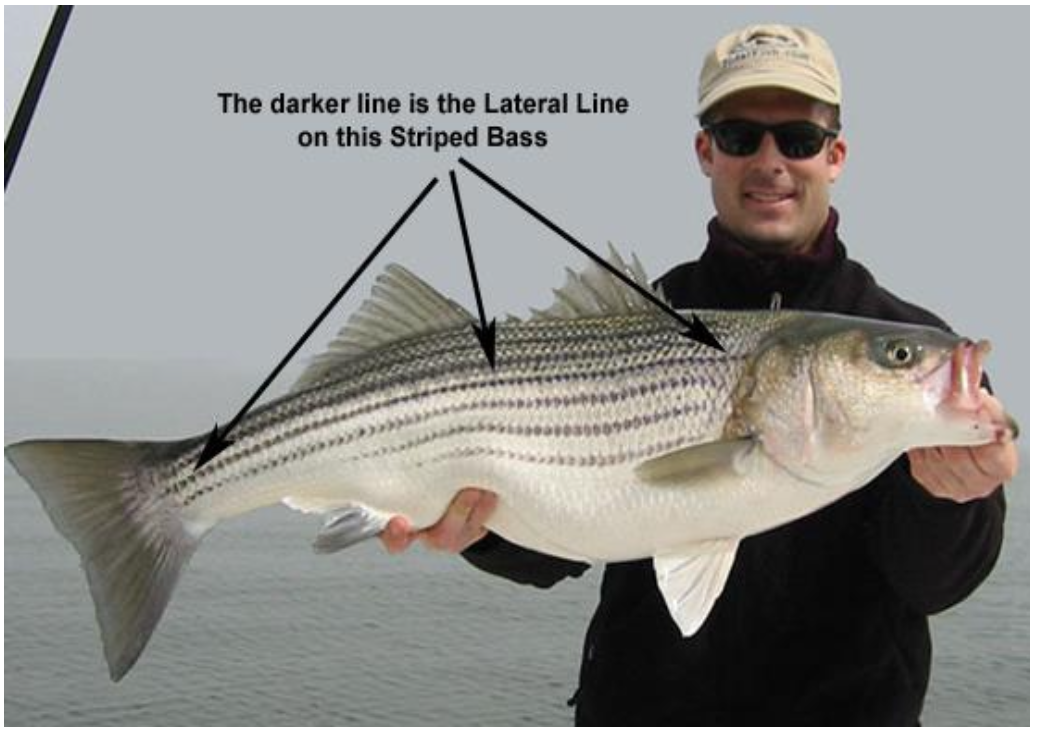
\includegraphics[width=5cm]{lec8/figures/fisch.png}
    \hfill
    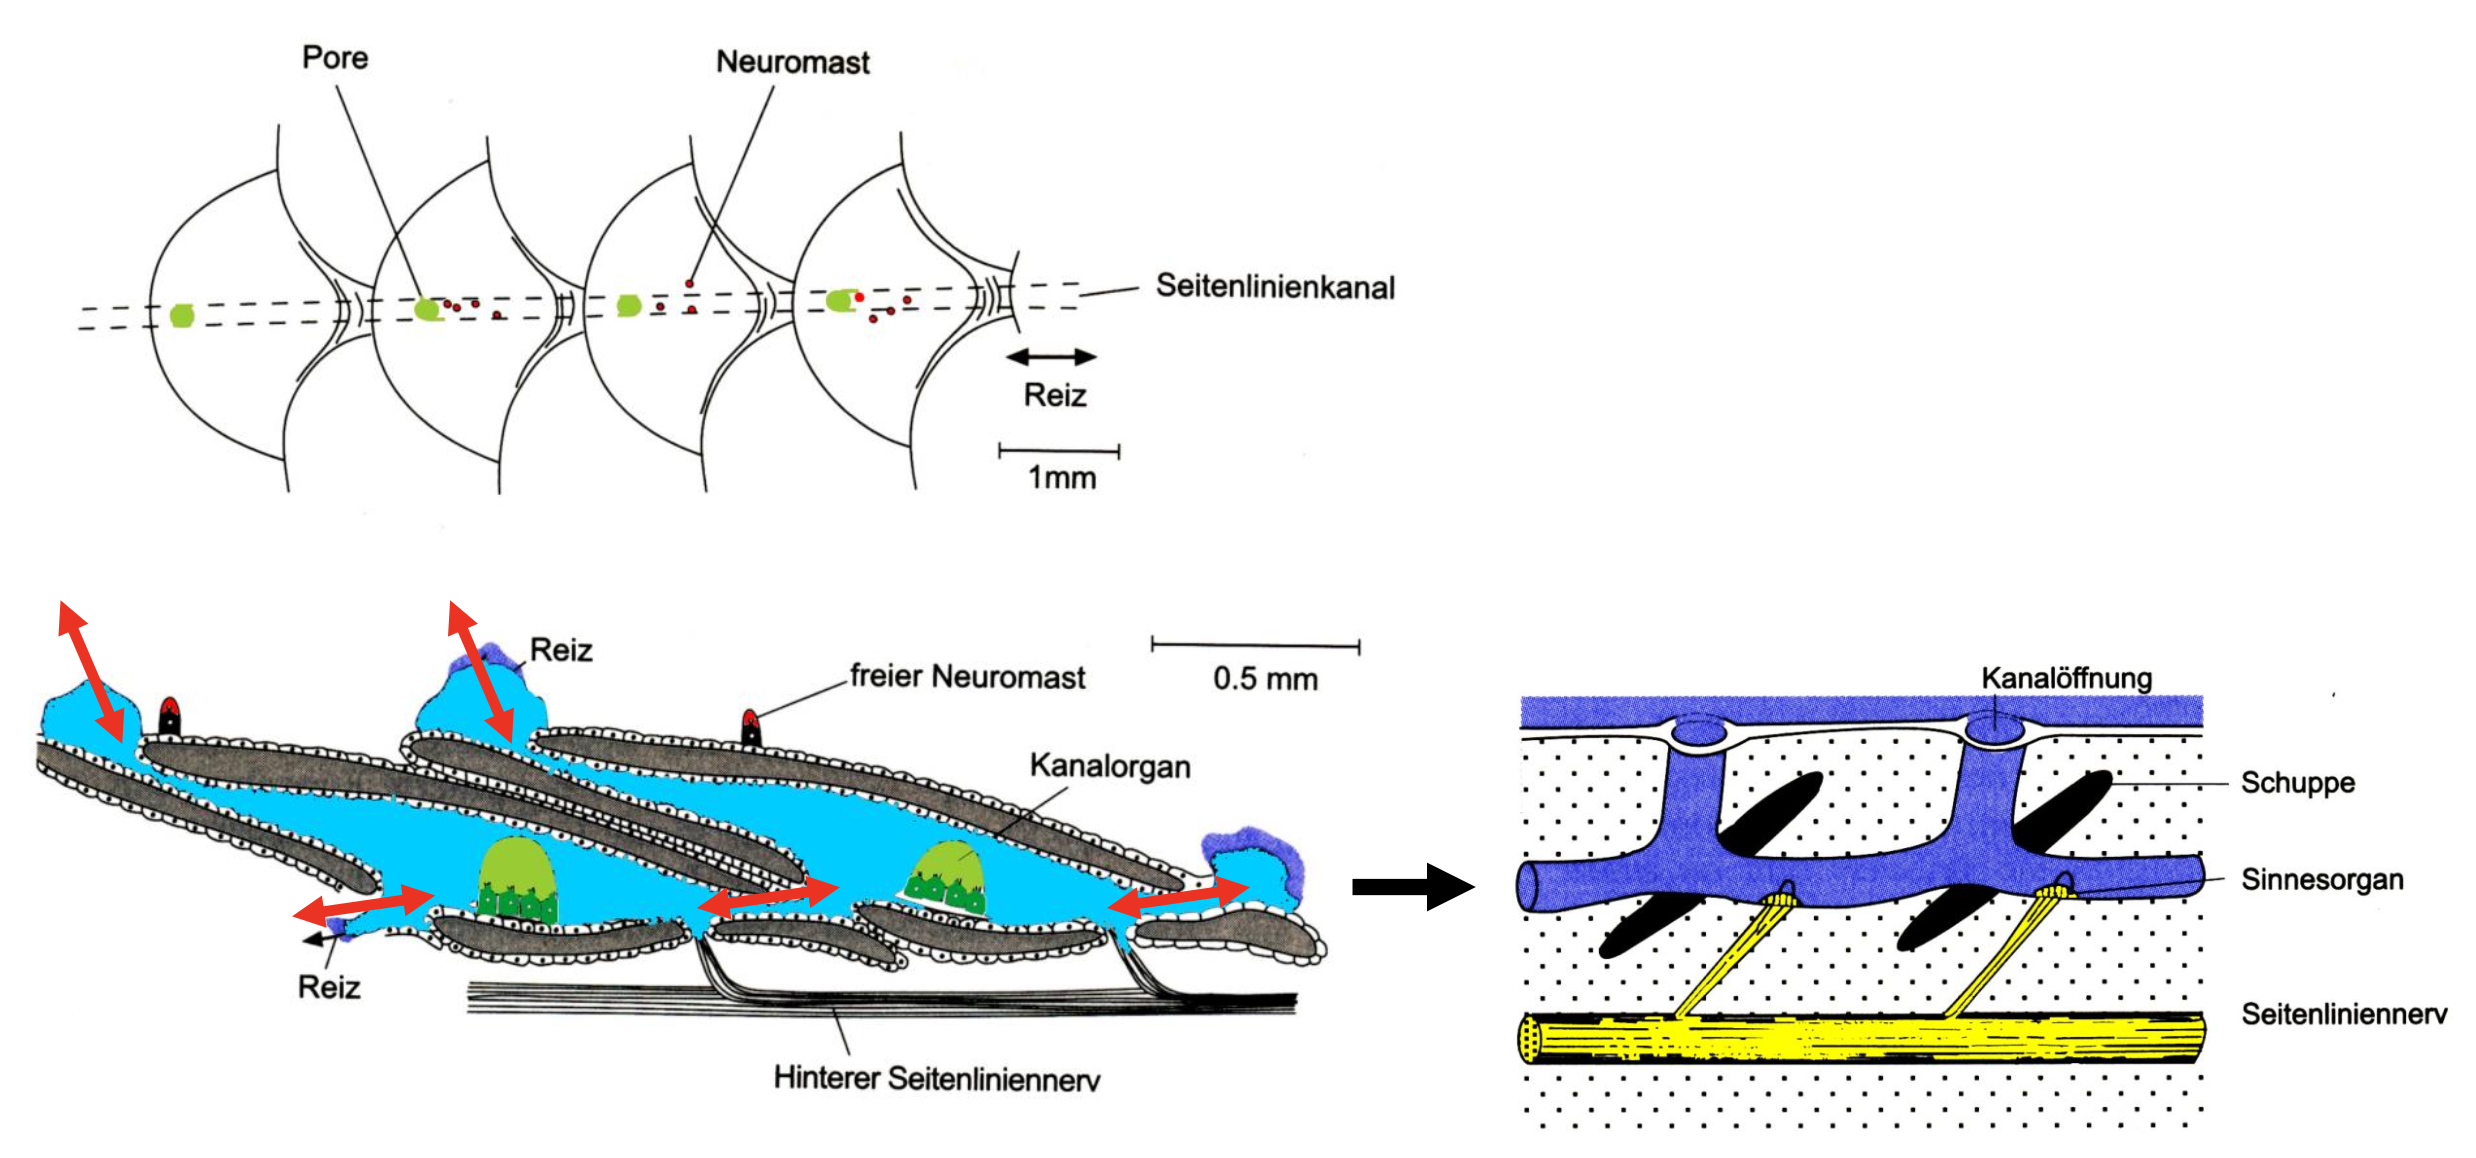
\includegraphics[width=11cm]{lec8/figures/seitenliniensystem.png}
    \\
    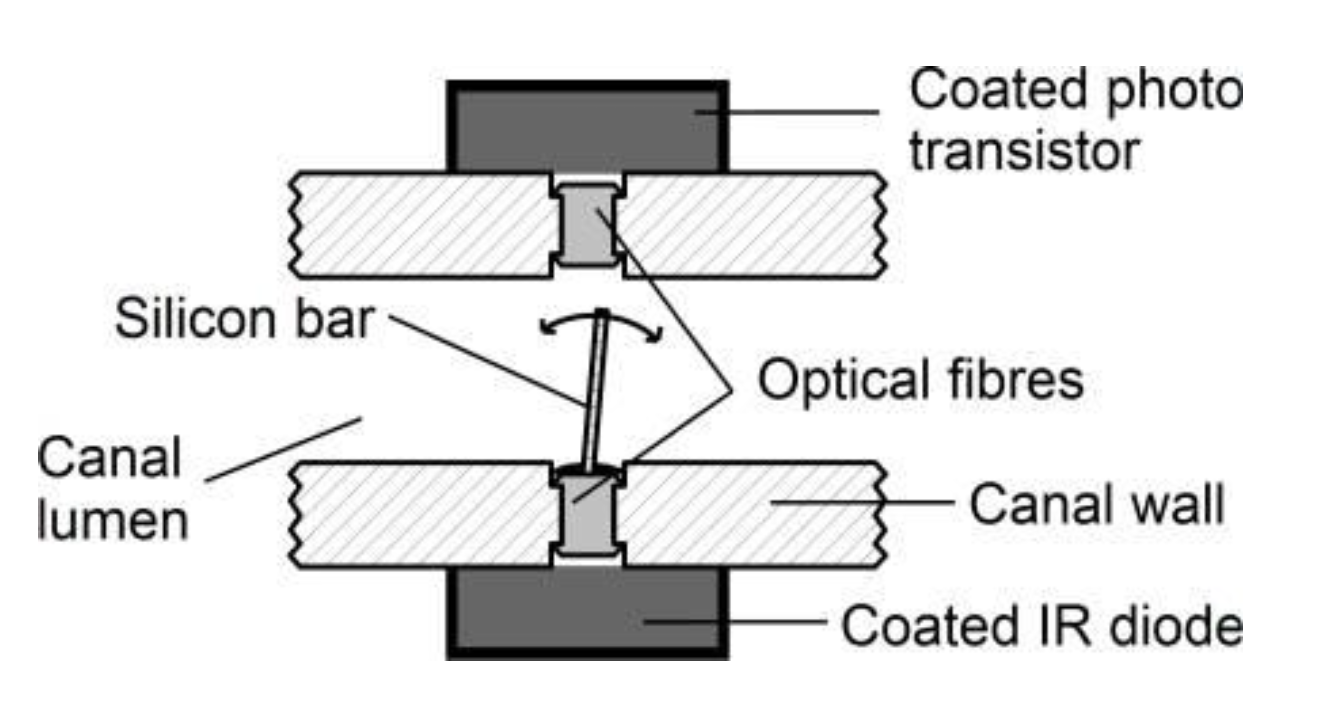
\includegraphics[width=5cm]{lec8/figures/mechanirezeptor.png}
\end{center}

\paragraph{Elektroortung bei Fischen} Hierbei haben die Rezeptoren sich vermutlich aus den Seitenlinienorganen entwickelt \dangersign. Die Voraussetzung ist ein leitendes Medium, z.B.\ Meerwasser. Spannungspotentiale steuern bspl.\ Muskelbewegungen in Lebewesen und erzeugen dadurch elektromagnetische Felder in der Umgebung. Haie oder Rochen besitzen Lorenzinische Ampullen am Kopf, über die sie diese Felder wahrnehmen und die Beute dann \textbf{passiv elektro-orten} können.

\paragraph{Starkelektrische Fische} Der Zitteraal, Zitterrochen und Zitterwels können elektrische Impulse (bis zu $500V$ und $0.83A$ beim Zitteraal) aussenden, um Räuber zu lähmen und Beute \textit{aktiv elektro-zu-orten}. \textbf{Wie generieren die Fische dieser hohen Spannungen \dangersign?} ``Zurückgebildete'' Muskelzellen bauen bei Aktivierung durch das Nervensystem Spannungspotentiale auf der Rückseite der Zelle auf (kontrahieren dann aber nicht wir herkömmliche Muskelzellen) $\rightarrow$ siehe im Bild unten. Da die Gegenseite der Muskelzelle isoliert ist, ergibt sich extrazellulär eine Nettospannung. Durch eine Reihenschaltung vieler Muskelzellen, können hohe Gesamtspannungen erreicht werden.

\begin{center}
    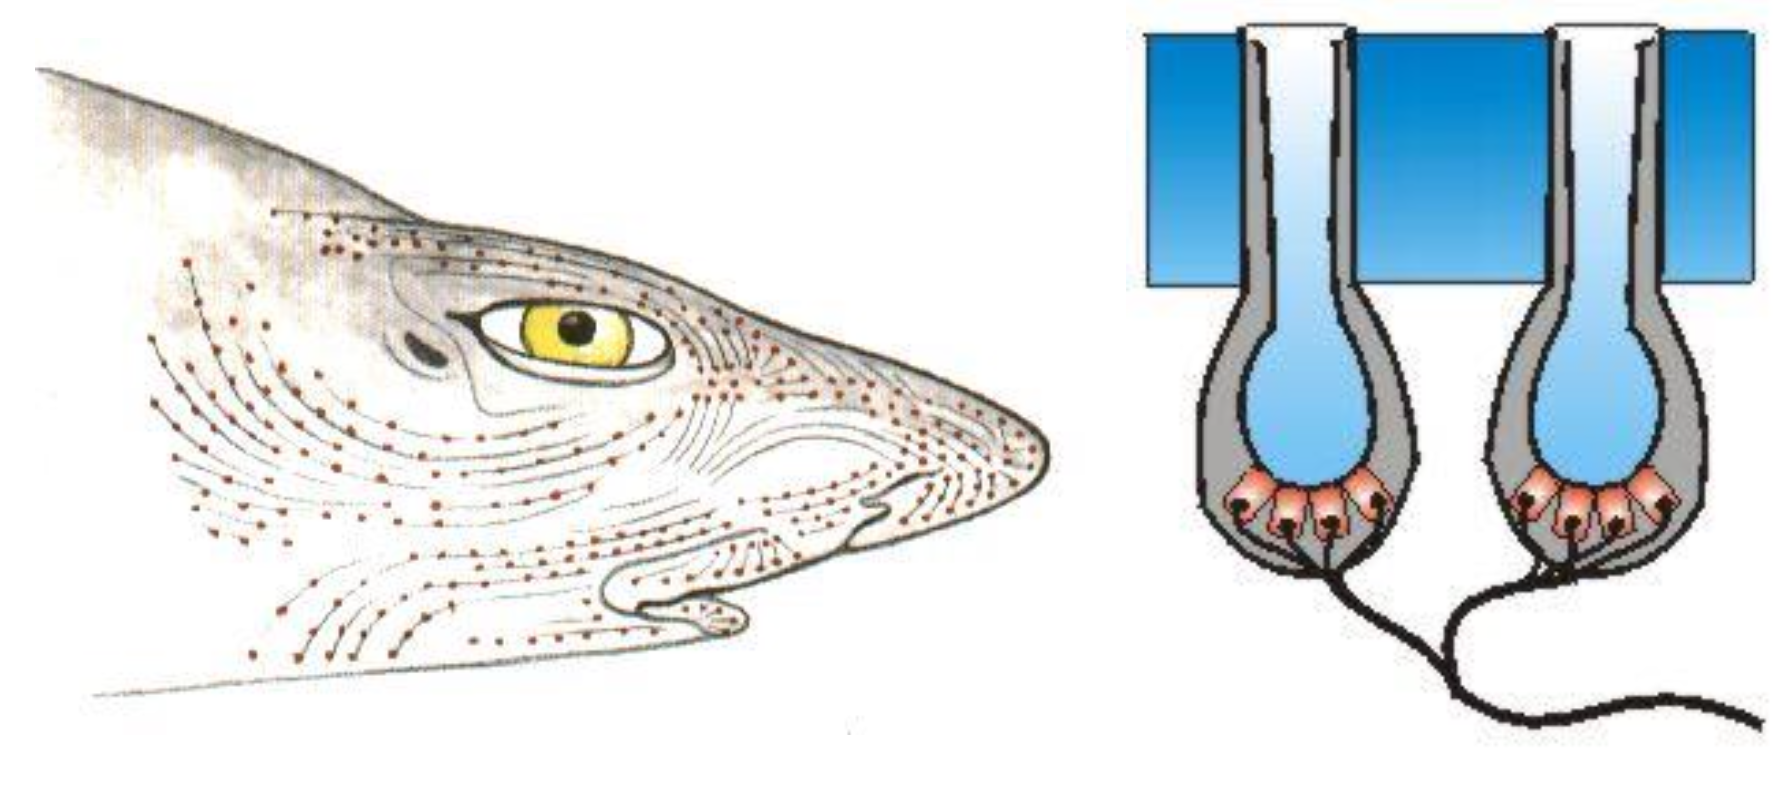
\includegraphics[width=7cm]{lec8/figures/hai.png}
    \hfill
    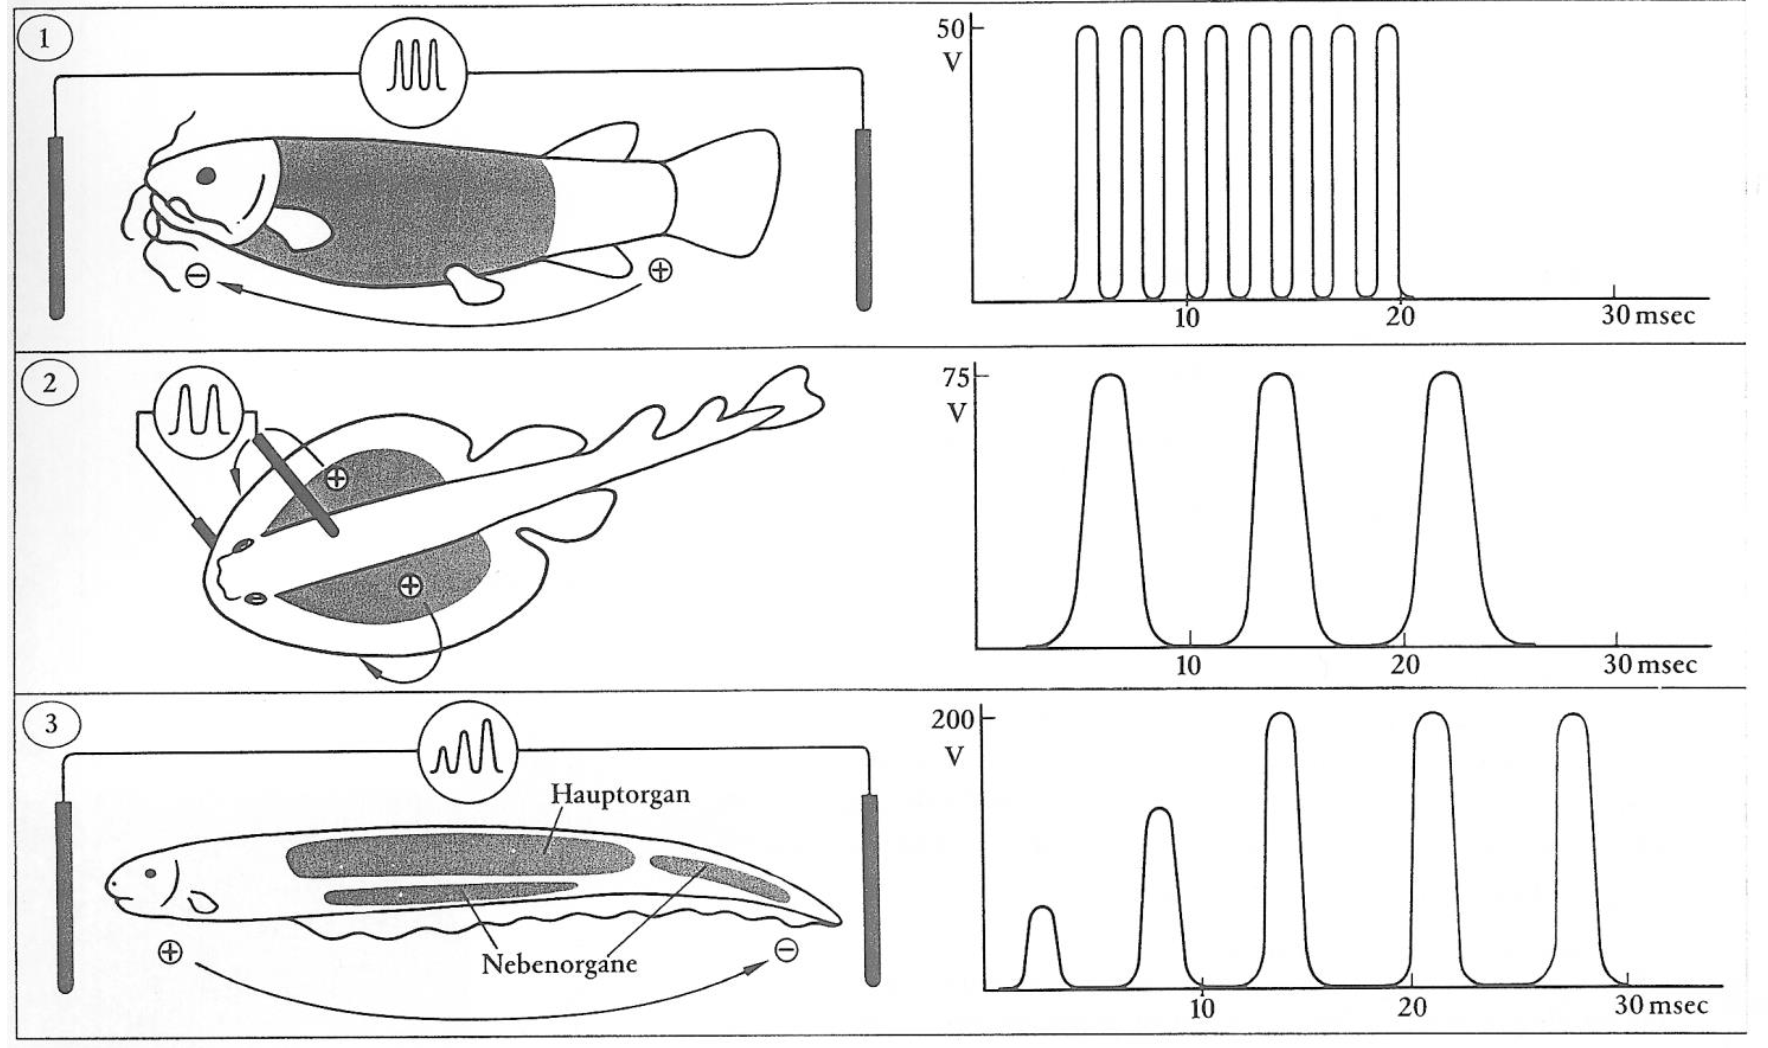
\includegraphics[width=6cm]{lec8/figures/starkelektrisch.png}
    \\
    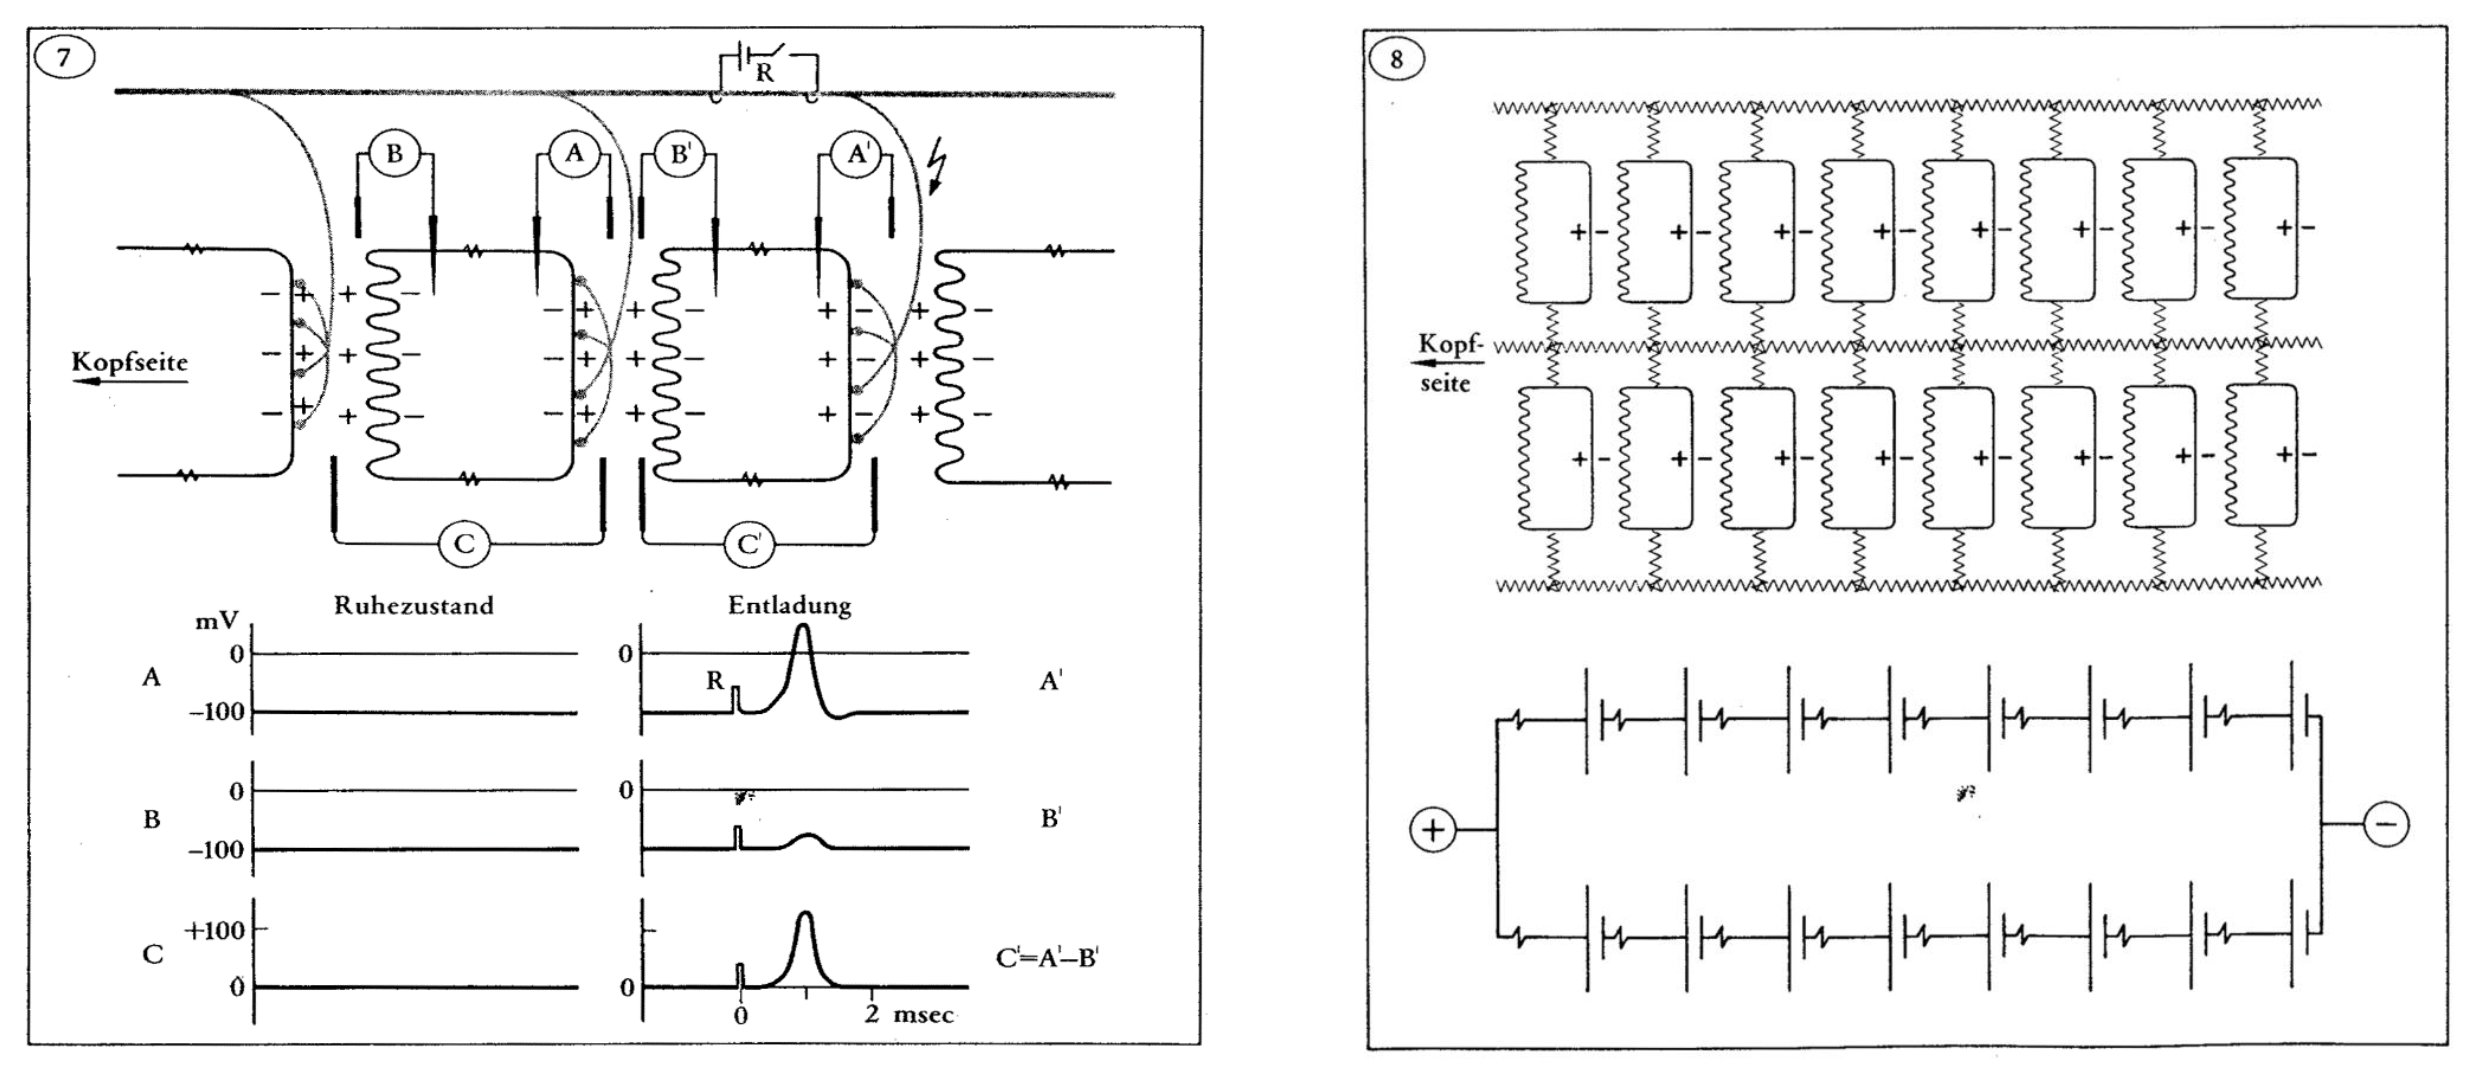
\includegraphics[width=11cm]{lec8/figures/muskelzellen.png}
\end{center}

\paragraph{Schwachelektrische Fische} Entladungen haben niedrige Leistung und erfolgen oft spontan und ausdauernd. Dabei dient das elektrische Feld der Kommunikation (Erzeugung eines eigenen elektrischen Feldes mit bestimmter Frequenz) und der Orientierung (Ein elektrisches Feld wird erzeugt und aus der Verzerrung des Feldes durch gute und schlechte elektrische Leiter in der Umgebung die Umgebung „errechnet“). Diese Fische kommen in trüben Wasser oder Wasser mit vielen Turbulenzen vor und bewegen sich nicht durch Schwanzschlag fort, sondern durch undulierende Bewegung (langsame vor- und zurück-Bewegungen zur Stabilisierung des erzeugten Feldes).
\\\\
\textit{Bionische Anwendung} \dangersign: Bei der Ateriosklerose kommt es zur Verengung von Blutgefäßen durch Ablagerungen (Plaques), wodurch Herzinfakte hervorgerufen werden können. Da sich durch die Ablagerungen die Leitfähigkeit der Gefäßwand verändert, können die \textbf{Plaques mithilfe der aktiven Elektroortung erkannt} werden.


\begin{center}
    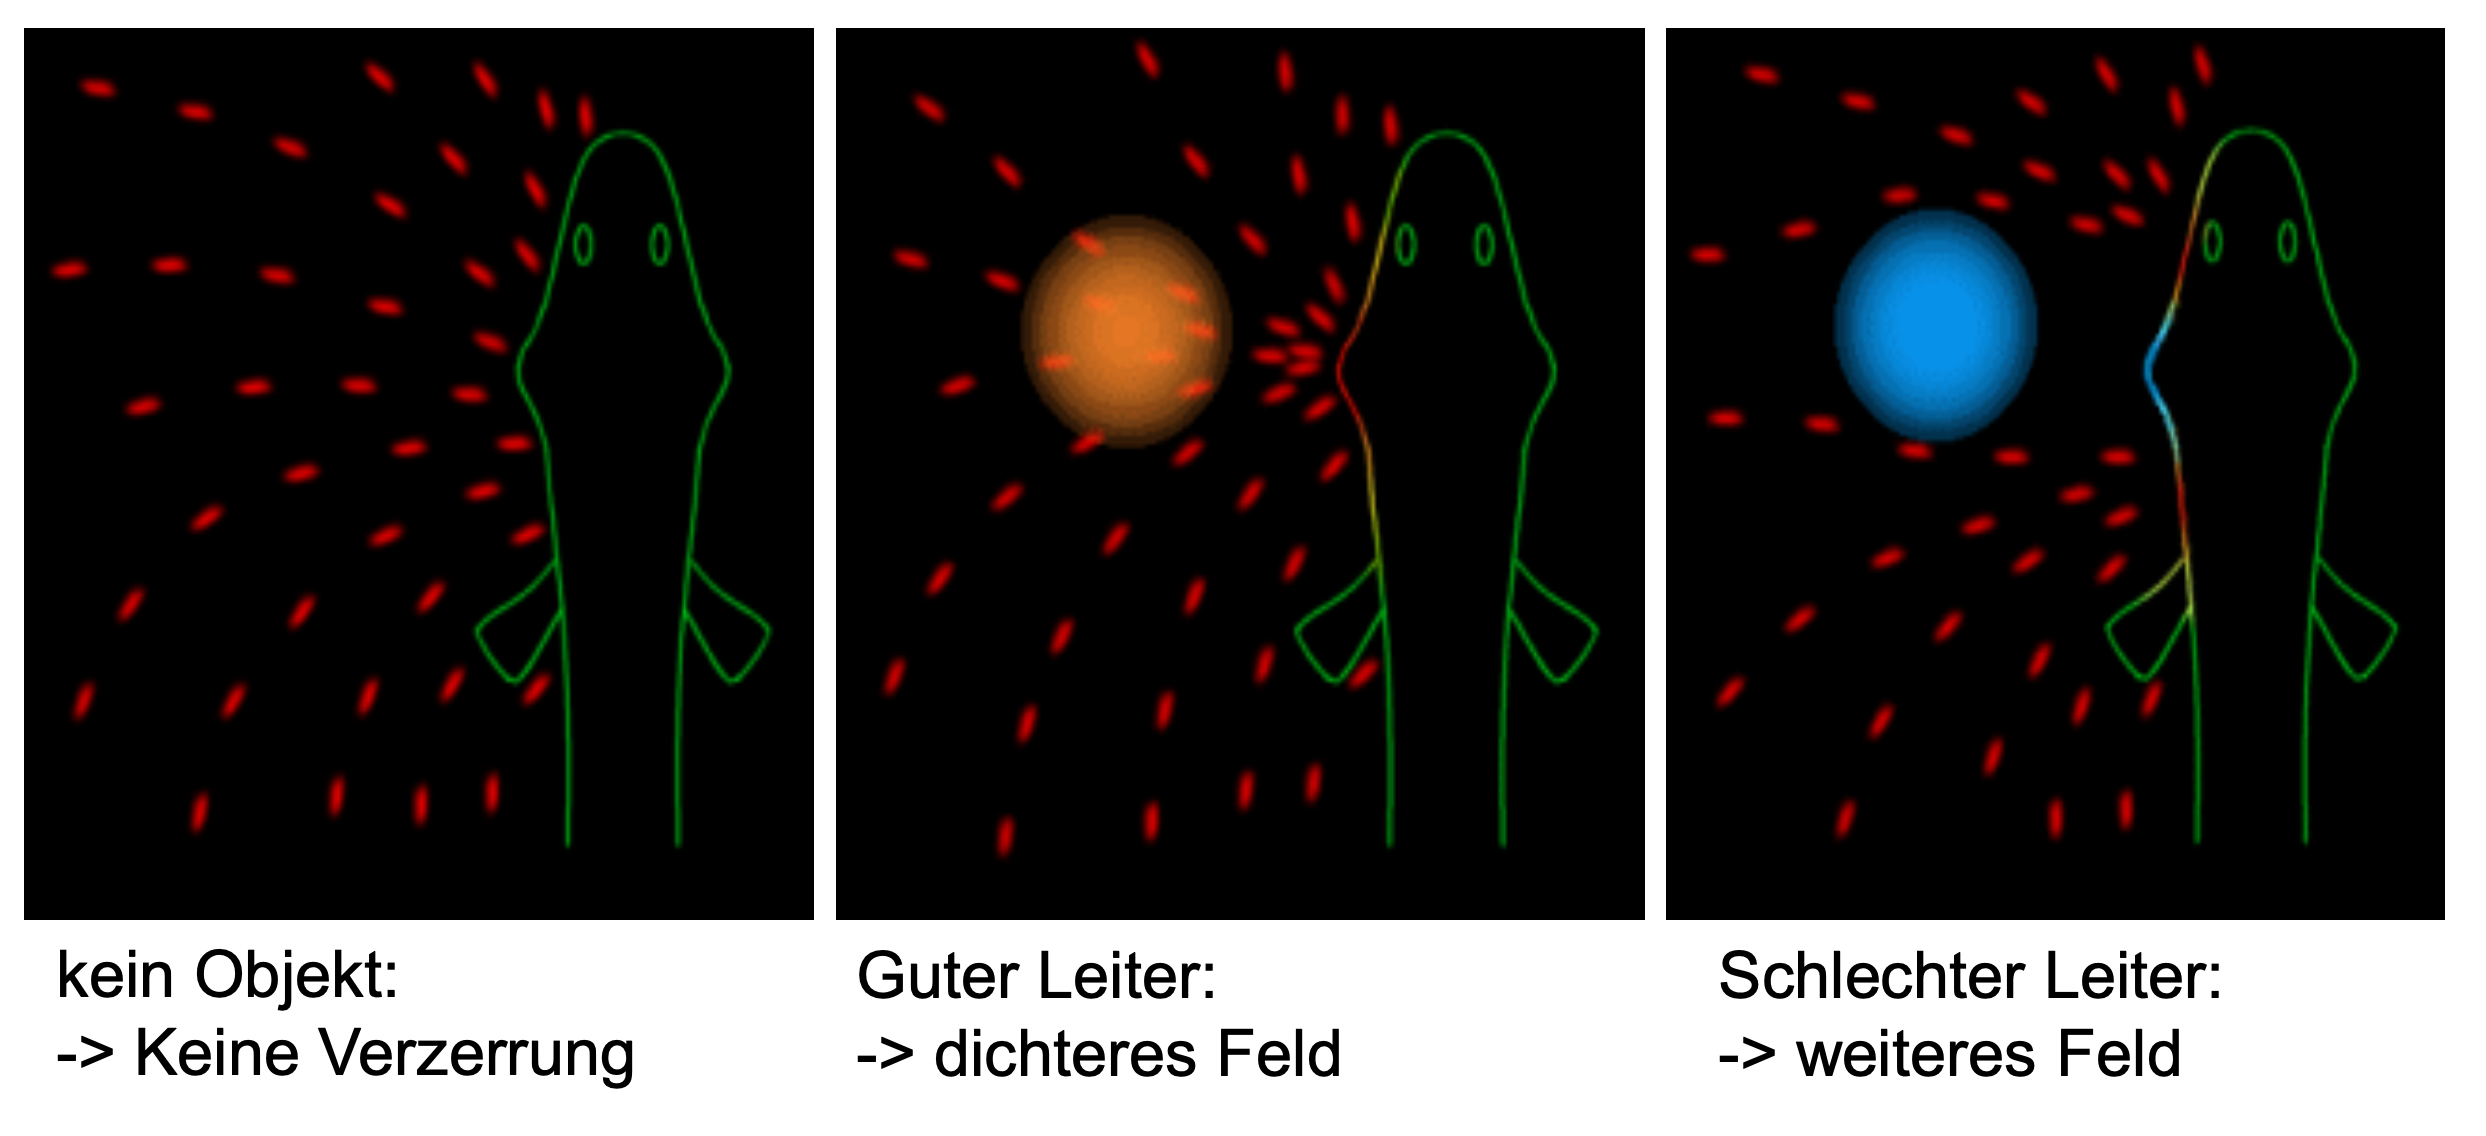
\includegraphics[width=8cm]{lec8/figures/leiter.png}
    \hfill
    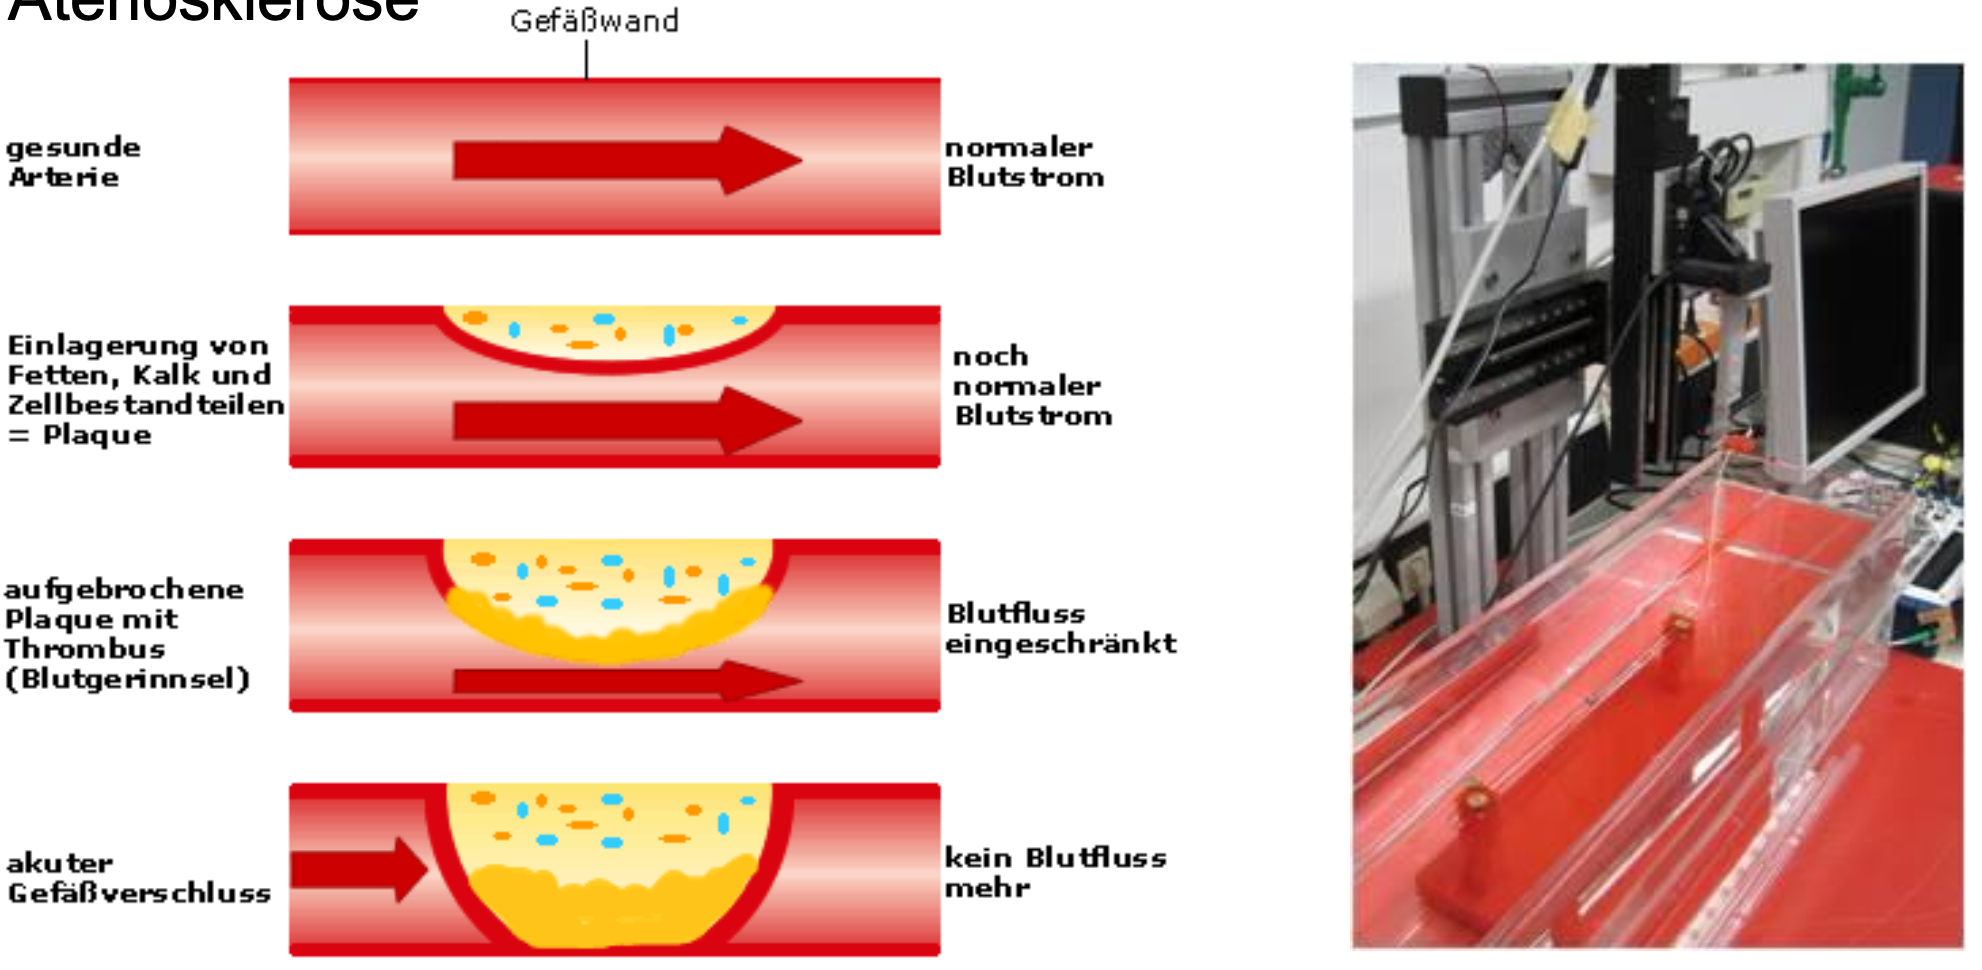
\includegraphics[width=8cm]{lec8/figures/plaques.png}
\end{center}